\chapter{Hardware Specification \& Design}
This chapter of the report focuses on creating a comprehensive set of specifications for the computer
to be built as a part of the project and then provides a detailed listing of the design choices made to satisfy
the specifications provided. Since the design will be based on Bean Eater's 8-bit breadboard computer \cite{eater2019breadboard}, but it will also include parts of SAP-2 and SAP-3 \cite{malvino1992digital}. Most specification criterions will be phrased as additions and enhancements to the existing designs.

\section{Specification Guidelines}
The specifications which are about to be presented serve the purpose of adding functionality to the 8-bit breadboard computer such
that its educational potential is harnessed more effectively, while at the same time avoiding over-complication and over-extensions
of scope. As such, it makes sense to list some of the features which will \emph{fall out of the scope} of this build for practical
and time considerations.
\begin{itemize}
  \item Interrupts and Interrupt handling
  \item Processes (The computer will only run one process, there will be no threading interface/ no operating system)
  \item Floating-Point operations
  \item Support for any kind of advanced in-hardware operations (for example encryption)
  \item Native support for signed integers over 16 bits
  \item Graphical User Interfaces (GUIs)
  \item Input through traditional peripheral (mouse and keyboard)
\end{itemize}

\section{Major Architecture Changes}
The computer should broadly follow the architecture o the 8-bit computer designed by Malvino and Brown \cite{malvino1992digital} and built by Bean Eater \cite{eater2019breadboard}. The major architectural difference should be \emph{the extension to 16-bit words}.
Since the word length of the computer should be 16 bits, its bus and most of its modules should be extended to accommodate this extra capacity.

\subsection{Operational Enhancments}
Besides Addition and Subtraction, the computer should also implement \emph{bit-shifting} (both left and righ). Bit-shifting is a crucial operation which is very often performed to increase the efficiency of certain operations (for example, multiplication and division by 2 can be expressed in binary as a left or a right shift of 1 bit)

\subsection{I/O Enhancements}
Currently, the only way to provide input to the 8-bit computer is by \emph{manually} programming each memory address through dip-switches. This is slow, clunky and prone to errors. There should exist a mechanism to quickly program the computer, for example through an external \emph{microcontroller} like an Arduino. Besides this, there should also exist a way for the computer to request input \emph{while executing} from an external device like a microcontroller.
Similarly, to provide persistence to the values from calculated by the computer, instead of being able to display only one value at a time, the computer should also have the ability to communicate with an existing external device like a separate microcontroller, providing it with the values it has calculated. In turn, the microcontroller a the be connected to a regular personal computer and then programmed to display those values to the screen. Besides this, the computer should have a display capable of displaying
more than 4 characters and more than just numbers.

\subsection{Stack Operations}
The addition of a stack pointer would make subroutines, calls to subroutines and callbacks significantly easier. An effective
stack pointer just has to have the option to increment and decrement, in contrast to a simple program counter which just increments.
With this functionality, return addresses can be pushed on and popped off of the memory stack whenever they are required.

\subsection{Expanded Random Access Memory}
Eater's implementation has a very limited address space (4 bit address, which equates to 16 addresses). While from a theoretical
point of view, this is as close to a Turing Machine as a supercomputer with terrabytes of RAM (an ideal Turing Machine should have infinite memory), a more reasonable amount of memory (in the kilobytes range) would allow for far greater flexibility in software
applications. For this computer, a 16K memory (\(2^{10} * 16\), or 10 bit address space) should be sufficent.

\subsection{Memory Layout}
Due to the added features, the memory layout of the 16-bit breadboard computer needs to be re-worked. As such, the following
layout is proposed:
\begin{itemize}
  \item From 0x000 to 0x1FF: Program Text
  \item From 0x200 to 0x3EF: Variables and Data
  \item From 0x3F0 to 0x3FF: Stack
\end{itemize}

\section{16-bit Breadboard Computer Layout}
Based on the previous specification, the computer to be built in this report should contain the following modules and
have the following physical layout:

\begin{figure}[h]
  \centering
  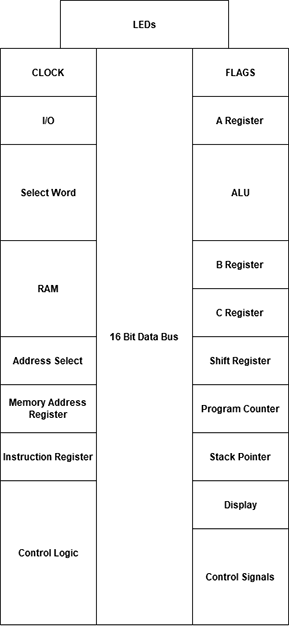
\includegraphics{16-bit-layout}
  \caption{High Level Module Overview and Layout of the 16-bit Breadboard Computer}
  \label{16-bit-layout}
\end{figure}
\clearpage

The updated computer specification contains the following modules, each of which will be followingly discussed in later sections:
\begin{enumerate}
  \item Common Data Bus \ref{common-data-bus}
  \item Data Bus LEDs \ref{data-bus-leds}
  \item Clock \ref{clock}
  \item A Register \ref{a-reg}
  \item B Register \ref{b-reg}
  \item Arithmetic-Logic Unit (ALU) \ref{alu}
  \item Flags Register \ref{flags}
  \item C Register \ref{c-reg}
  \item Shift Register \ref{shift-reg}
  \item Random Access Memory (RAM) \ref{ram}
  \item Program Counter \ref{pc}
  \item Stack Pointer \ref{stack-pointer}
  \item Display \ref{display}
  \item I/O \ref{io}
  \item Memory Address Register \ref{mar}
  \item Instruction Register \ref{ir}
  \item Word Selector \ref{word-select}
  \item Address Selector \ref{addr-select}
  \item Control Logic \ref{control-logic}
  \item Control Signals \ref{control-sigs}
  \label{module-list}
\end{enumerate}

\subsection{Common Data Bus} \label{common-data-bus}
The Common Data Bus acts as the communication medium of the computer. Drawing a parallel between \emph{computer design}
and \emph{human anatomy}, the data bus acts like the circulatory systems. It ensures all other components are connected
and can talk to each other. The Common Data Bus should be 16 bits wide, since the final system should have a word length of
16 bits. Since all other modules connect to the Data Bus, it makes sense to have it located centrally, between all other modules.
This way, no module has to have particularly long wires to interface with the Bus.

\subsection{Data Bus LEDs} \label{data-bus-leds}
This modules is as simple as it gets. It should be composed of just 16 LEDs, or Light Emitting Diodes, one on each Data Bus line,
so that whatever gets asserted at a certain point in time on the Bus can be visible. Besides this, it can also contain pull-down
resistors to ensure that, if no module asserts anything on the bus, it should default to low, or a logic 0.

\subsection{Clock} \label{clock}
The clock acts as the heart of the system. It provides a pulse under the form of a square wave, based on which all other components
do their job. The clock signal should be distributed to all other modules. Besides providing the square wave clock pulse an inverse,
or counter clock pulse should be available, as well as the ability to change the frequency and to completeley stop the square wave
and replace it with a manual button press for demonstrational and debugging purposes.
Finally, the clock should take in one signal as input, namely halt, or \emph{HLT},
which should completeley stop the clock regardless of operating mode. This will allow the computer to halt execution
if, for example, the program is finished. \\
\textbf{$Input\:Control\:Signals:\:HLT$} \\
\textbf{$Output\:Control\:Signals:\:CLK, \overline{CLK}$}

\subsection{A Register} \label{a-reg}
The A register is a 16-bit memory storage module. It should implement three functions. First, when its \emph{AI}
(A Register In) signal goes high, it should latch in the contents of the data bus on the rising edge of the next clock pulse.
The second function is to output its contents to the bus when its \emph{$\overline{AO}$} (A Register Out) signal goes low. Finally,
if the \emph{$\overline{RST}$} (Reset) signal goes low, it should clear out its contents and latch in a 0 on all bits. Additionally,
the A register should have a direct 16-bit connection to the \emph{Arithmetic Logic Unit}, or ALU \ref{alu}. \\
\textbf{$Input\:Control\:Signals:\:CLK,\:AI,\:\overline{AO},\:\overline{RST}$}
\textbf{$Direct\:Connection\:to:\:ALU$}

\subsection{B Register} \label{b-reg}
Similarly to the A Register, the B Register should store 16 bits of data from the bus. It should have similar control signals,
\emph{BI, BO} and \emph{RST}, which perform equivalent functions. It should also have a direct 16-bit connection to the \emph{ALU}
\ref{alu}.
\textbf{$Input\:Control\:Signals:\:CLK,\:BI,\:\overline{BO},\:\overline{RST}$}
\textbf{$Direct\:Connection\:to:\:ALU$}

\subsection{Arithmetic Logic Unit} \label{alu}
The Arithemtic Logic Unit, or ALU, is the module responsible with data procesing. It takes the contents from\emph{both A and B
registers} \ref{a-reg} \ref{b-reg} directly and adds them up. Is the \emph{SU} (Subtract) signal is provided, the contents of the
B Register \ref{b-reg} will be subtracted from the contents of the A register. If the \emph{$\overline{\varepsilon O}$} (Sum Out)
is taken low, the contents of the  ALU will be asserted on the data bus. The ALU also has a direct connection to the Flags Register
\ref{flags}. Over this connection, the ALU should provide three flags:
\begin{itemize}
  \item Parity Flag: whether the \emph{Least Significant Bit} is 0 or 1
  \item Zero Flag: wheter the content of the ALU is 0
  \item Carry Flag: wheter the result of the operation of the ALU is cannot be expressed within 16 bits
\end{itemize}
\textbf{$Input\:Control\:Signals:\:\varepsilon\:O,\:SU$}
\textbf{$Direct\:Connection\:to:\:A\:Register,\:B\:register,\:Flags\:Register$}

\subsection{Flags Register} \label{flags}
The Flags Register is essential towards ensuring the Turing completeness of the computer being built. Based on the state of the
flags, the computer can make branch decisions, which reflect the fact that Turing machines can make selective decisions based
on the symbol it has just read.
Essentially, the flags register serves the purpose to latch in the three flags provided by the ALU \ref{alu}: the Parity Flag, the
Zero Flag and the Carry Flag. When the \emph{FI} (Flags In) signal is taken high, on the next clock pulse it should latch in the
contents of those flags. Besides this, the Flags Register should clear its contetns when the \emph{$\overline{RST}$} (Reset) signal
is taken low. There is a direct connection between the Flags Register and the Control Logic module, as the flags play a role in
deciding what to do next. \\
\textbf{$Input\:Control\:Signals:\:CLK,\:FI$}
\textbf{$Direct\:Connection\:to:\:ALU$}

\subsection{C Register} \label{c-reg}
The C Register serves as a general purpose 16-bit register. It has signals similar to the other two registers, A \ref{a-reg} and
B \ref{b-reg}. When \emph{CI} (C Register In) goes high, on the next clock pulse the register should latch in the data word
asserted on the bus in its storage. IF \emph{$\overline{CO}$} (C Register Out) goes low, the register should assert its contents
on the data bus. IF \emph{$\overline{RST}$} (Reset) goes low, it should clear its contents and latch in onyl zeroes. There should
be no direct connection between the C register and any other registers. \\
\textbf{$Input\:Control\:Signals:\:CLK,\:CI,\:\overline{CO},\:\overline{RST}$}

\subsection{Shift Register} \label{shift-reg}
The Shift Register is the other module of the 16-bit breadboard computer capable of conducting data processing tasks. First and
foremost, it should act as a normal register, so it should latch in the bus contents on the next clock pulse if the \emph{SI}
(Shift Register In) signal goes high, asserts its contents to the bus if \emph{$\overline{SO}$} goes low, and clears it contents
if \emph{$\overline{RST}$} goes low. Besides this, if \emph{SFL} (Shift Left) goes high, on the next clock pulse it should shift its
contents to the left by one bit and insert a 0 at the least significant bit of the data word. Similarly, if \emph{SFR}
(Shift Right) goes high, on the next clock pulse it should shift its contents one bit to the right and insert a 0 at the most
significand bit of the data word. \\
\textbf{$Input\:Control\:Signals:\:CLK,\:SI,\:\overline{SO},\:SFL,\:SFR,\:\overline{RST}$}

\subsection{Random Access Memory (RAM)} \label{ram}
Random Access Memory, or RAM, is the equivalent of the tape on a Turing machine. It can be read from and written to, and it should
be large enough to accommodate algorithms, data and variables; all at the same time. Memory is organised in addresses. Each address
should store one 16-bit word of memory. A 10-bit address is deemed to be sufficent, so the computer should have a
\(2^{10}*16 = 16K\) memory space. The RAM module should also have a direct connection to the \emph{Address Selector}
\ref{addr-select} and to the the \emph{Word Selector} \ref{word-select}. The Address Selector serves a 10-bit address to the
memory, while the word selector serves a 16-bit data word to the RAM. If the \emph{RI} (RAM In) signal goes high, on the next clock
pulse the RAM Module should latch in the data word served by the word selector at the address provided by the address
selector. If the \emph{RO} signal goes low, the RAM module should assert the data word stored at the address provided by the
address selector on the data bus. Additionally, based on two control signals originating from toggle switches, \emph{PROG} and
\emph{ARDUINO}, the signal which governs the RAM writes can be changed. If \emph{PROG} is low, that means the computer is in run
mode, and the \emph{RI} signal controls writes. If \emph{PROG} is high, then the computer is in programming mode, and the
write signal is chosen based on the \emph{ARDUINO} signal. If \emph{ARDUINO} is low, then the writes are manually controlled
using a simple push button. If it is high, then an external \emph{Arduino Mega} \cite{arduino2020mega} controls the writes to
memory using a signal called \emph{$ARDUINO_WRITE$}. \\
\textbf{$Input\:Control\:Signals:\:CLK,\:RI,\:RO,\:PROG,\:ARDUINO,\:ARDUINO_WRITE$} \\
\textbf{$Direct\:Connection\:to:\:Word\:Selector,\:Address\:Selector,\:Arduino Mega$}

\subsection{Program Counter} \label{pc}
The Program Counter serves the purpose of keeping track of the current address which should be executed. As such, it should
be a 10-bit register, to ensure coverage of the entire address space of the computer. If the \emph{CE} (Counter Enable) signal
goes high, on the next clock cycle the program counter should count up one in binary from the value it has currently latched
in its storage and then latch this new value in. If the \emph{$\overline{JMP}$} (Jump) signal goes low, on the next clock pulse the
program counter should latch in whatever value is asserted on the 10 loweest bits of the bus in its register. If
\emph{$\overline{CNT_O}$} (Counter Out) goes low, the value latched in the program counte should be asserted on the data bus.
If \emph{$\overline{RST}$} (Reset) goes low, the program counter should clear out its contents and latch in zeroes on all bits. \\
\textbf{$Input\:Control\:Signals:\:CLK,\:CE,\:\overline{JMP},\:\overline{CNT_O},\:\overline{RST}$}

\subsection{Stack Pointer} \label{stack-pointer}
Tha stack pointer should essentially be a register holding a 10-bit address, but accepting only a small subsection of the address
space (from 0x3F0 to 0x3F). This means that the stack should be 16 addresses tall. If the \emph{$\overline{ST_I}$} (Stack Increment)
signal goes low, on the next clock pulse, the stack pointer should increment by one. If \emph{$\overline{ST_D}$} (Stack Decrement)
goes low, the stack pointer should decrement by one on the next clock pulse.
On \emph{$\overline{ST_J}$} (Stack Jump) going low, on the next clock pulse the stack pointer should latch in the address asserted
on the bus in its register, assuming it is a valid stack address. If \emph{$\overline{ST_O}$} goes low, the stack pointer should
assert the address it has stored out on the bus. Finally, if \emph{$\overline{RST}$} (Reset) goes low, the stak pointer should reset
to zero. \\
\textbf{$Input\:Control Signals:\:CLK,\:\overline{ST_I},\:\overline{ST_D},\:\overline{ST_J}, \overline{ST_O},\:\overline{RST}$}

\subsection{Display} \label{display}
The Display module is the main way through which the computer can interface with the user. It should have the ability to display
both alfanumeric characters and digits and it should feature at least 2 lines of 16 characters each. When the \emph{OUT} (Output)
signal goes high, the display should take a word of data from the bus and interpret it as the next character to be written to the
screen. \\
\textbf{$Input\:Control\:Signals:\:OUT$}

\subsection{I/O} \label{io}
Besides a display, the computer should also feature a bidirectional interface to another mirocontroller. In this case,
the interface should be to an \emph{Arduino Mega} \cite{arduino2020mega}. If the \emph{$\overline{E}$} (Enable) signal goes low,
based on the \emph{$R/\overline{W}$} (Read/Write) signal, the computer should interact with the Arduino. If the
\emph{$R/\overline{W}$} signal is high the computer should read a word of data from the arduino, so that word of data should be
asserted on the bus. If the \emph{$R/\overline{W}$} signal is low, the Arduino should read a word of data from the bus (and
consequently displayed to the user). \\
\textbf{$Input\:Control\:Signals:\:\overline{E},\:R/\overline{W}$} \\
\textbf{$Direct\:Connection\:to:\:Arduino Mega$}

\subsection{Memory Address Register} \label{mar}
The memory address register, or MAR, is a 10 bit register. It connects directly to the address selector \ref{addr-select} and
there is no other way to get the information latched into it. If the \emph{MI} signal goes high, on the next clock pulse the MAR
will latch into its storage the 10 least significant bits asserted on the bus. if \emph{$\overline{RST}$} goes low, the MAR will
clear its contents and write zeroas to all 10 bits. \\
\textbf{$Input\:Control\:Signals:\:CLK,\:MI,\:\overline{RST}$} \\
\textbf{$Direct\:Connection\:to:\:Address\:Selector$}


\subsection{Instruction Register} \label{ir}
The Instruction Register, or IR, is a 16-bit register which holds the next instruction to be processed. It is special in that
its most significant 6 bits have a different meaning. They represent the opcode for the current instruction and are directly
connected to the Control Logic module \ref{control-logic}. When the \emph{II} (Instruction Register In) signal goes high, on the
next clock pulse the instruction register should latch in the data word asserted on the bus in its storage. If the
\emph{$\overline{IO}$} (Instruction Register Out) signal goes low, the register should assert its least significand 10 bits to the
bus. If \emph{$\overline{RST}$} (Reset) goes low, the instruction register should reset and latch in zeroes on all 16 bits. \\
\textbf{$Input\:Control\:Signals:\:CLK,\:II,\:\overline{IO}$} \\
\textbf{$Direct\:Connection\:to:\:Control\:Logic$}


\subsection{Word Selector} \label{word-select}
The Word Selector is a special module, in that it serves the purpose of selecting between different sources of data and feeding
them into the RAM module \ref{ram}. There are three possible sources of data
\begin{enumerate}
  \item The Data Bus
  \item Dip Switches
  \item An Arduino Mega
\end{enumerate}
The Data Bus is the first and most straight forward data source. A 16-bit data word can be taken from the bus and then passed on
to memory. The second source are Dip Switches. Dip Switches are rows of small binary switches, which can be used to manually feed
binary data into a digital system. The last possible source of data is an arduino mega. The choice of data to be fed forward is
governed by two control signals, \emph{PROG} and \emph{ARDUINO}. If \emph{PROG} is low, data from the data bus will be selected,
regardless of the state of \emph{ARDUINO}. If \emph{PROG} is high, that means that the computer is in programming mode. In this
mode, the data source depends on the \emph{ARDUINO} control signal. If this signal is high, then data will be fed forward from
an external Arduino Mega \cite{arduino2020mega}. If it is low, then a series of 16 dip switches will be used to manually program
the computer.  \\
\textbf{$Input\:Control\:Signals:\:PROG,\:ARDUINO$} \\
\textbf{$Direct\:Connection\:to:\:RAM,\:Arduino\:Mega$}

\subsection{Address Selector} \label{addr-select}
Similar to the Word Selector \ref{word-select}, the Address Selector selects between different address sources to provide a 10-bit
address to  the RAM module \ref{ram}. There are three possible data sources:
\begin{enumerate}
  \item The Memory Address Register \ref{mar}
  \item Dip Switches
  \item An Arduino Mega
\end{enumerate}
The choice of data source is defined by two control signals, \emph{PROG} and \emph{ARDUINO}. If \emph{PROG} is low, then the
computer is in run mode and the address latched in the \emph{MAR} \ref{mar} is fed forward to RAM. If it is high, then that means
the computer is in programming mode and the address choice is governed by the \emph{ARDUINO} control signal. If it is low, then
the memory address will be manually chosen using a series of 10 Dip Switches. If it is high, then an external
Arduino Mega \ref{arduino2020mega} will be the address source. \\
\textbf{$Input\:Control\:Signals:\:PROG,\:ARDUINO$}
\textbf{$Direct\:Connection\:to:\:RAM,\:Arduino\:Mega$}

\subsection{Control Logic} \label{control-logic}
To draw another parallel to human anatomy, the control logic module can be thought of as the ~~brain`` of the computer.
It takes in the 6-bit opcode from the Instruction Register \ref{ir}, the 3 flags from the Flags Register \ref{flags}, as well as
a 3 bit number representing the ~~step`` of the current instruction which is to be executed and decides based on these pieces
of information which control signals to keep active on the next clock cycle. It also maintains an internal 3 bit counter which
counts on the inverted clock or counter clock signal to provide the 3-bit step. \\
\textbf{$Input\:Control\:Signals:\:\overline{CLK}$}
\textbf{$Output\:Control\:Signals\: HLT,\:\overline{RST},\:AI,\:\overline{AO},\:BI,\:\overline{BO},\:\overline{\varepsilon O},\:SU,\: FI,\:CI,\:\overline{CO},\:SI,\:\overline{SO},\:SFL,\:SFR,\:RI,\:RO, \:CE, \:\overline{JMP},\: \overline{CNT_O},\:\overline{ST_I},\:\overline{ST_D},\:\overline{ST_J},\:\overline{ST_O},\:OUT,\: \overline{E},\:R/\overline{W},\:MI,\:II,\:\overline{IO}$}
\textbf{$Direct connection to: Instruction Register, Flags Register$}


\subsection{Control Signals} \label{control-sigs}
The Control Signals Module is used to visualise which control signals are active at any given time. This module should
essentially consist of a labeled LED on each control signal.

\section{Specification Conclusion}
This concludes the specification phase of the project. The next step is to design each module to this specification.

\section{Design}
This section of the report focuses on the design process for the individual modules of the 16-bit breadboard computer.
The goal is to satisfy all specification criterions designated in the last section, while also adhering to the general goal
and philosophy of the project as close as project. First of all, the design process will be documented and analysed. After that,
the tools used to facilitate the design will be presented. Finally, each module design will be presented and scrutinized.

\subsection{How to design a 16-bit computer module}
In order to successfully come up with a design for a computer module while also meeting the specification outline and
keeping the schematics as simple as possible, a simple yet effective design process has been implemented. It consists
broadly of 4 distinct steps:
\begin{itemize}
  \item Chip Discovery
  \item Chip Analysis
  \item Chip Selection
  \item Schematic Creation
\end{itemize}

\subsection{Chip Discovery and Analysis}
The first step towards the design of a 16-bit computer module is the \emph{integrated circuit/IC/chip} discovery and analysis phase.

\paragraph{Why use Integrated Circuits/Chips?}
Since the general goal of the project is to produce a Turing complete computer which is as simple as possible to understand
and also relies as little as possible on any other form of abstraction, one might argue that using integrated circuits, or chips,
woud be against that goal. While this argument is theoretically correct, it doesn't take into account any practical considerations.
The lowest level of the technology stack from which one could go ahead and phisically construct a computer would probably be
the transistor. That being said, trying to implement any computer, let alone a 16-bit computer with many different modules, would
be next to impossible to successfully do within the time frame of this project and also without a team of people. The physical
scale would be many, many times what the scale of the computer built in this project is and the amount of errors which would arise
from connecting individual transistors together by hand would probably be so large, that one would quickly lose interest in
finishing the build. As such, simple integrated circuits pose themselves as a great compromise. These circuits, which usually
implement simple logic functions, like \emph{AND, OR, Inverter, etc.}, or even a little bit more complex functions,
like \emph{registers or binary adders}, can each contain tens to hundreds of individual transistors. That being said, they should
all be simple enough so thatthe functionality provided by each chip should be \emph{understandable down to the transistor level}.

\paragraph{Understanding Integrated Circuits}
While this may sound daunting at first, it can actually be relatively straight forward. Individual logic gates are each made up of
a few transistors. For example, Ben Eater has created an excellent YouTube tutorial on how to create logic gates out of transistors
\cite{eater2015logicgates}. Armed with this knowledge, we can now approach the datasheet of a particular circuit we intend to use.
For example, on page 2 of the datasheet of the \emph{74LS157} \cite{74ls157} multiplexer chip, we can find the logic diagram.
By analysing the logic diagram and calculating boolean outputs based on arbitrary inputs and then comparing the results
to the truth table of the chip provided on the first page of the datasheet, one can verify that the chip actually implements its
specified interface in a logical manner. This can be applied to all chips which are considered to be potential building blocks
for a module, as long as the individual chip complexity is relatively limited.

\subsection{Where to look for Integrated Circuits}
There are three main sources of chips which where consulted when conducting chip discovery. The first one was the Wikipedia list
of chips from \emph{7400} family \cite{wikipedia74lslist}. This particualr logic family was chosen because it is the most popular
and widley spread and adopted logic family in the world \cite{wikipedia74ls}. The second souce of chips, which served as a quick
reference, was Eater's part listing for his 8-bit breadboard computer build \cite{eater2020parts}. Since the 16-bit computer which
is to be built is largley based around the 8-bit computer built be Eater, many of the chips used in the 8-bit version will also
work in modules of the 16-bit version. Finally, for the few chips which were needed but weren't part of the 7400 family,
the websites of the retailers from which the chips were to be bought were searched. Two retailers were used, \emph{Mouser UK}
\cite{mouser} and \emph{Farnell UK} \cite{farnell}.

\subsection{Chip Selection}
Usually, the particular functionality of the module which is to be designed drastically boils down the list of potential chips.
For example, when designing a simple 16-bit register, like the \emph{A register} \ref{a-reg}, the \emph{74LS273} 8-bit flip-flop
\cite{74ls273} poses a great option. By just putting two \emph{74ls273} chips next to each other, most of the functionality of the
register has been designed. Whenever there is a need for extra functionality, for example in the case of the \emph{74ls273}
where there is no enable line, additional logic can be implemented using chips containing simple logic gates, like \emph{AND, OR,
NOT}. In this case, the clock signal can be AND'ed together with the \emph{AI} line to ensure that the register only reads from the
data bus when the control signal is set high.

\subsection{Schematic Creation}
With the right chips chosen for a module, the next step is to create a module schematic, which serves as a blueprint or design
document. The open-source computer-aided design software chosen to facilitate the creation of module schematics is \emph{KiCad}
\cite{kicad}. An overview of the application, as well as of the process of designing 16-bit computer modules with it will be
presented in detail in the next section.

\subsection{Electronic Design Tools with KiCad/Eeschema}
The main tool used to to design schematics for the 16-bit breadboard computer is \emph{KiCad} \cite{kicad}. KiCad is a broad and
mature electronics design software widley used in industry. It contains many tools which together from a tightly integrated
toolchain for designing complex electronics from the concept phase all the way to the printed circuit board. Since the goal of the
project is to build a computer on breadboards by hand and not create printed circuit boards, only the first step of the KiCad
pipeline has been used, namley \emph{Eeschema} \cite{eeschema}.

\paragraph{Eeschema}
\emph{Eeschema} is a electronic schematic computer design software. It is fully featured, easily accessible and has a relatively
shallow learning curve. By using \emph{Eeschema,} the entire module design process has been streamlined significantly.

\begin{figure}[h]
  \centering
  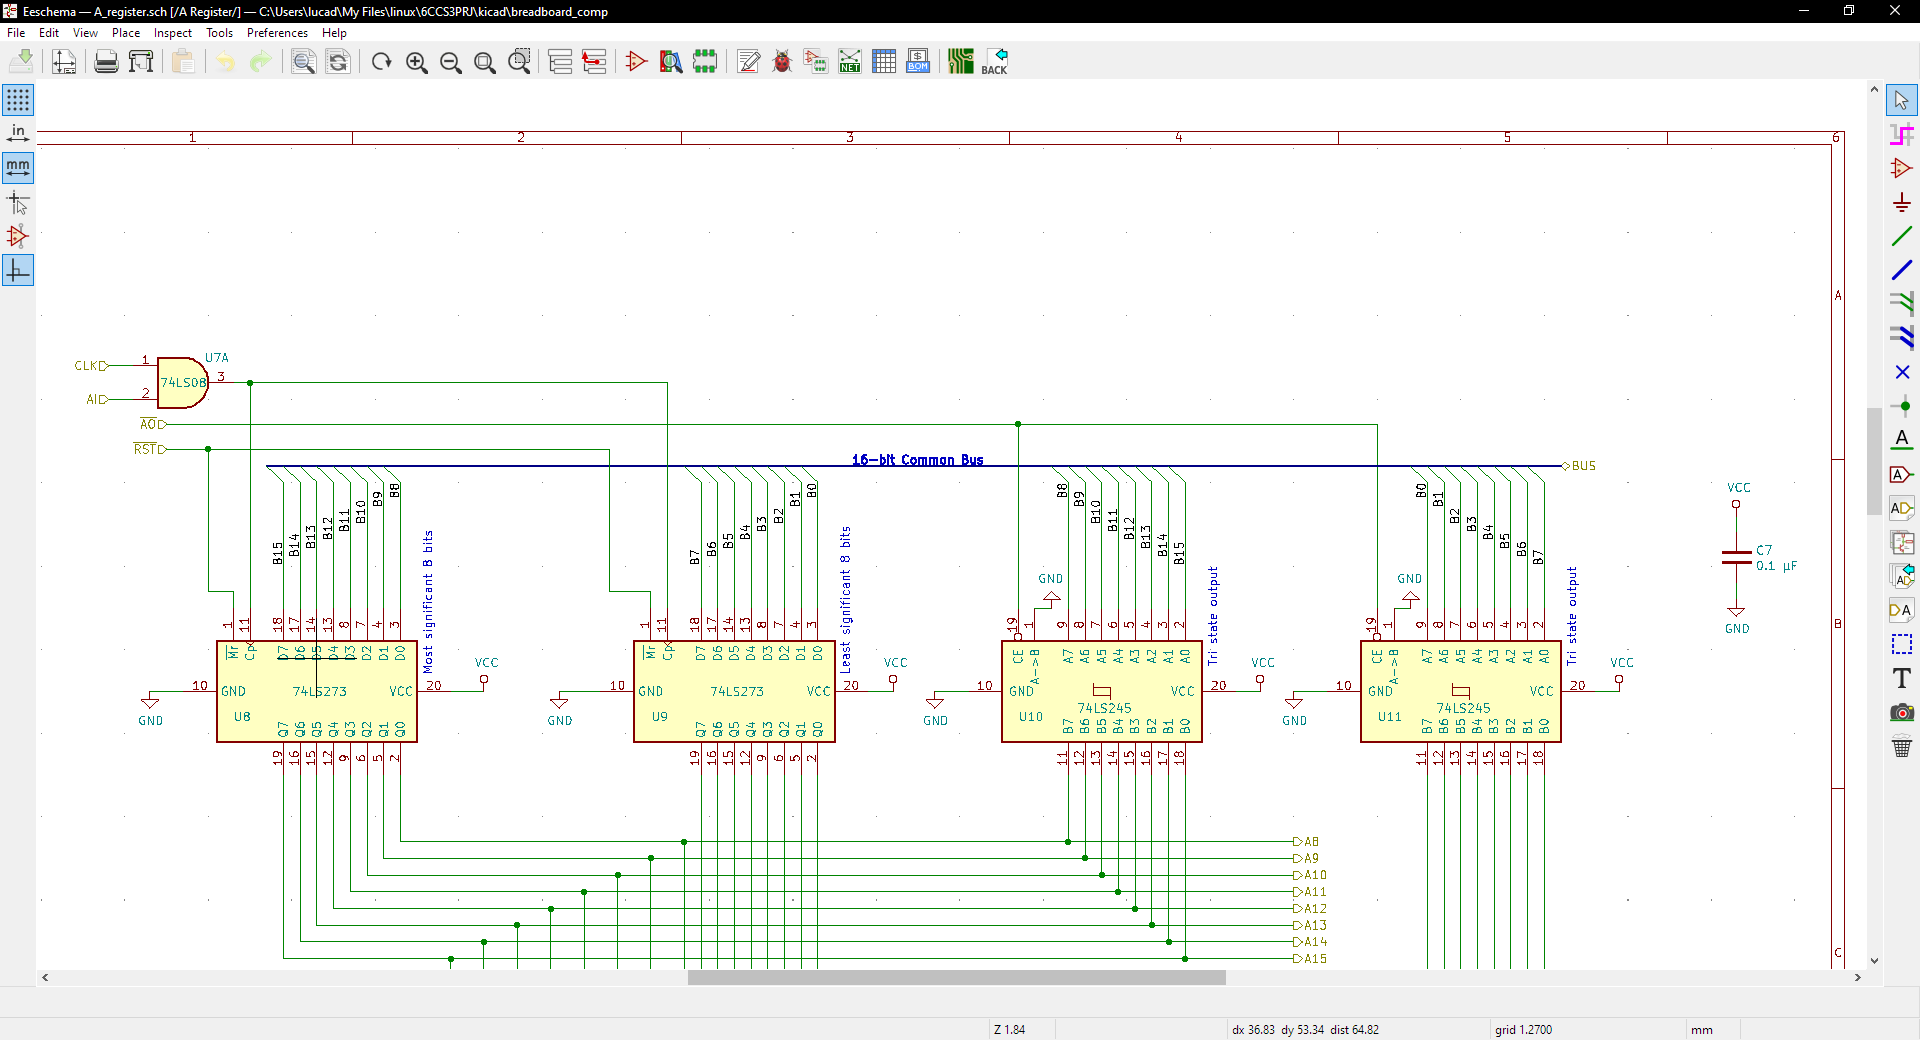
\includegraphics[scale=0.3]{eeschema}
  \caption{Eeschema Schematic Design software - part of the KiCad suite}
  \label{eeschema-interface}
\end{figure}
\clearpage

In the following paragraphs the most important features of Eeschema will be presented.

\paragraph{Intuitive Interface}
The graphical user interface provided by Eeschema is similar to many other widley used photo or video editing software packages.
As such, navigation is easy and intuitive. All tools and commands can be accessed both by pointer and keyboard, so one can become
proficient in whatever interface method is preferred. Drag and drop functionality allows the user to easily reposition misplaced
or misalligned circuits and components.

\paragraph{Hierarchical Sheets}
Hierarchical sheets is an Eeschema feature which allows one to embed entire schematics inside other schematics and seamlessly
transition between child and parent schematics. This is a great way to organise the modular design of the 16-bit breadboard
computer. Besides this, Eeschema offers the option to import input and output pins from the child schematic into the parent,
so that they can be connected to the wider circuit. This makes designing a high-level overview diagram significantly easier.

\paragraph{Bus connections}
Wiring up 16 separate wires which are connected to most modules as both input and output can be extremley tedious. Fortunatley,
\emph{Eeschema} offers the option to ~~bundle up'' mutliple wires as a single Bus and then have connections going in and out
of that single wire. Besides this, \emph{Eeschema} can resolve which pins are connected to which over the bus by use of labels
on the inputs and outputs \ref{ee-bus}.

\begin{figure}[h]
  \centering
  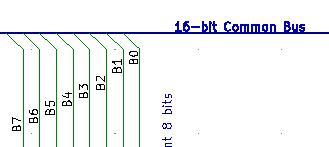
\includegraphics{ee-bus}
  \caption{Labeled Bus Connections in Eeschema}
  \label{ee-bus}
\end{figure}

\paragraph{Integrated Circuit Database}
\emph{Eeschema} ships with a pre-loaded database of commonly used chips and circuits, called the \emph{Symbol Library}.
This makes rapid schematic prototyping possible by just looking up potential circuits for the module and then dragging and dropping
them into the worksheet and then seeing if the connections would match up.

\begin{figure}[h]
  \centering
  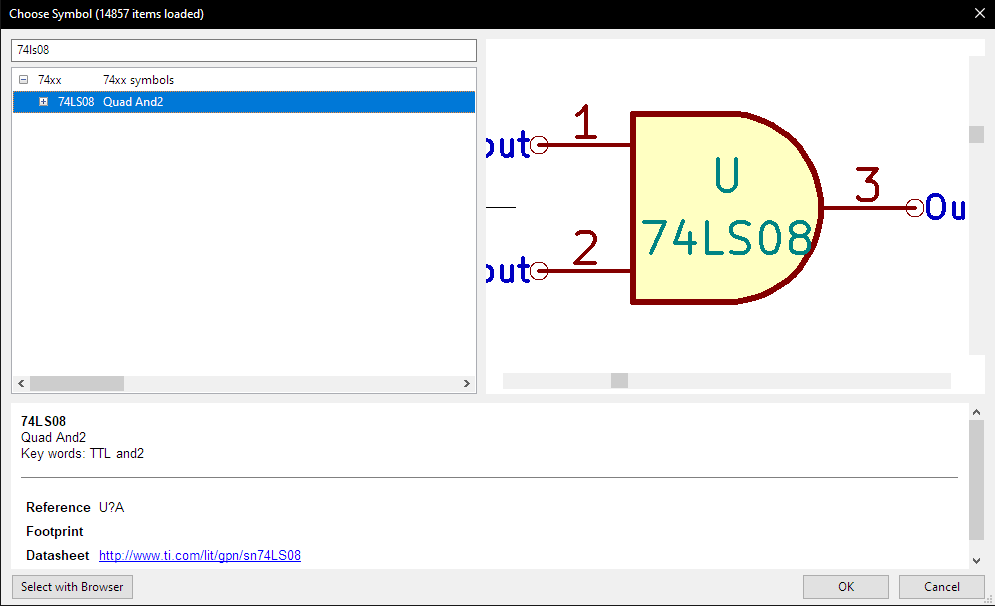
\includegraphics[scale=0.5]{ee-circuit-db}
  \caption{Component Database in Eeschema}
  \label{ee-circuit-db}
\end{figure}

\paragraph{Symbol Editor}
In the rare case where the \emph{Symbol Library} didn't contain a circuit needed for a module, \emph{Eeschema} provides
a simple circuit symbol editor. This ensures that the final schematics produced were accurate and reliable, regardless of wherer
the chip symbols were origianlly available in \emph{Eeschema} or not.

\begin{figure}[h]
  \centering
  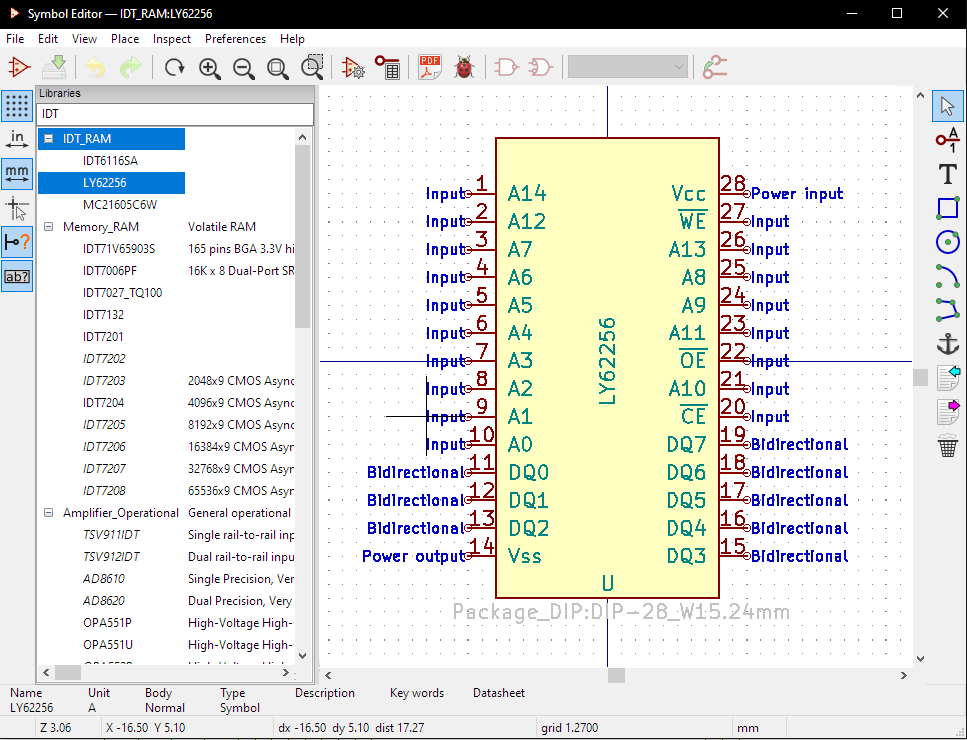
\includegraphics[scale=0.4]{ee-editor}
  \caption{Symbol editor in Eeschema}
  \label{ee-editor}
\end{figure}

\paragraph{Electrical Rules Check}
Besides providing an easy to use interface for designing accurate schematics, \emph{Eeschema} also offers active help in the
design process. By using the electrical rules checker, \emph{Eeschema} can check all connections against a user-defined set of
rules and report errors. This can be used to detect potetential human errors or even chip incompatibilities and resolve them
early on.

\begin{figure}[h]
  \centering
  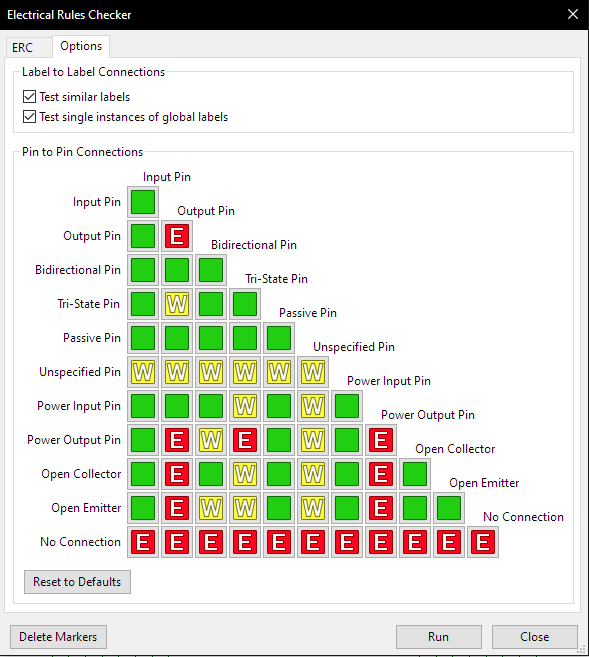
\includegraphics[scale=0.5]{ee-rules}
  \caption{The Eeschema Electrical Rules Checker}
  \label{ee-rules}
\end{figure}

\paragraph{Automatic Annotation}
When designing electrical circuits, it is common to use many identical or similar circuits next to one another. As such,
when actually building the circuit, one can be confused about which chip correlates to which symbol in the schematics.
To solve this, \emph{Eeschema} assignes a unique identifier, or annotation, to each symbol. This annotation process can be
done automatically.

\paragraph{Bill of Materials}
\emph{Eeschema} can also generate a bill of materials, or \emph{BOM}, based on all the symbols present in the schematic and
hierarchical schemaitcs. The BOM is essential towards ensuring that all needed components are purchased.

\begin{figure}[h]
  \centering
  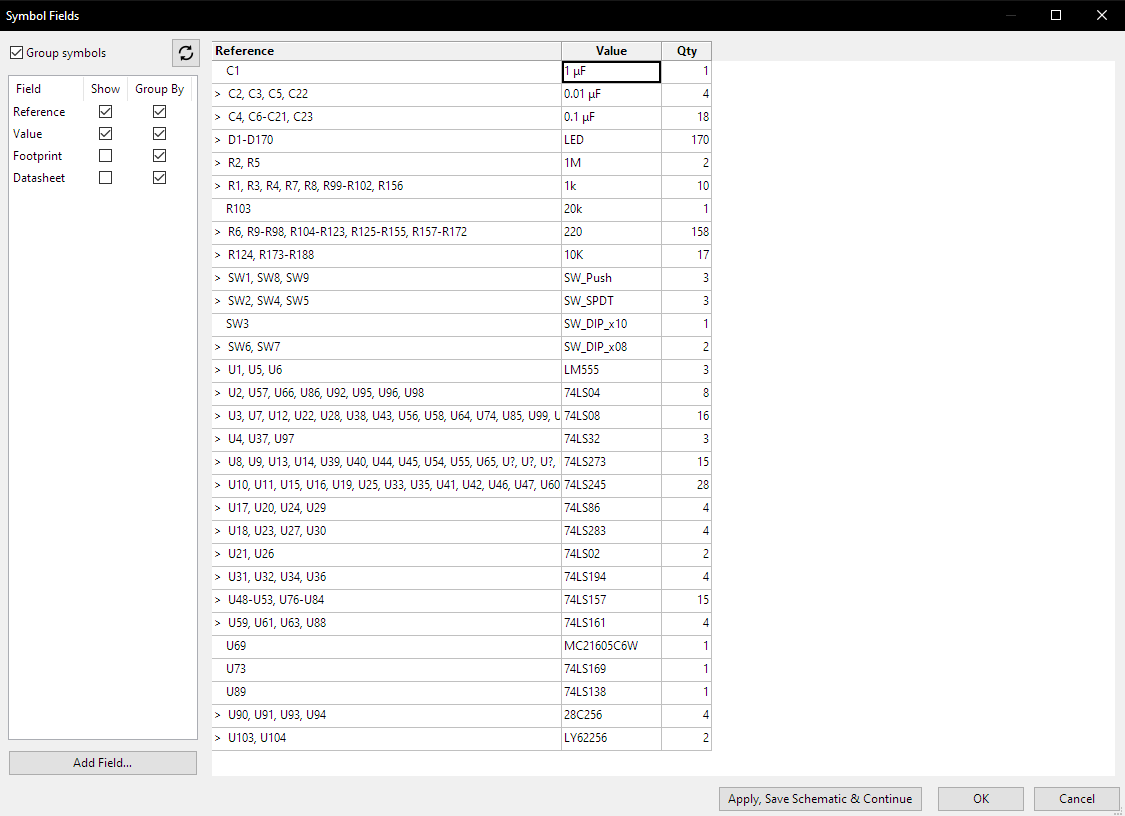
\includegraphics[scale=0.4]{ee-bom}
  \caption{Simple Bill of Materials generated by Eeschema}
  \label{ee-bom}
\end{figure}

\paragraph{PDF export}
Finally, Eeschema has been outfitted with an ~~Export to PDF'' option. This makes printing and compiling of the
schematics into other documents, like this report, significantly easier.

\subsection{Eeschema Design Process}
The following design process has been followed when creating schematics for a module as a part of the 16-bit breadboard
computer:
\begin{enumerate}
  \item Make an adequate chip selection
  \item Create a new hierarchial sheet and enter it
  \item Use the Symbol Editor to create chip symbols (in case the chips don't exist in the Symbol Library)
  \item Place all needed chips in the schematic
  \item Place all external control and I/O pins
  \item Connect all the pins apropiateley
  \item Leave the hierarchical sheet and import all I/O and control pins
  \item Run the automated annotation tool
  \item Run the electrical rules checker
  \item Correct any errors
\end{enumerate}

\subsection{Finalised 16-bit breadboard computer design and schematics}
The tools and processes discussed in the previous sections where extensivley used to produce the final schematics
for the 16-bit breadboard computer, which were used as templates for the physical implementation of the computer.
This section presents and discusses the schematics and the design decisions which were made during their creation.

\paragraph{High-Level Schematic}
The high-level schematic provides a layout and scale overview for the finished computer. It also contains the \emph{Data Bus LEDs}
module \ref{data-bus-leds}, as well as the actual \emph{Common Data Bus} \ref{common-data-bus}, to which all components connect.
Towards the bottom of the schematic the \emph{LEDs} module \ref{control-sigs} can also be found.

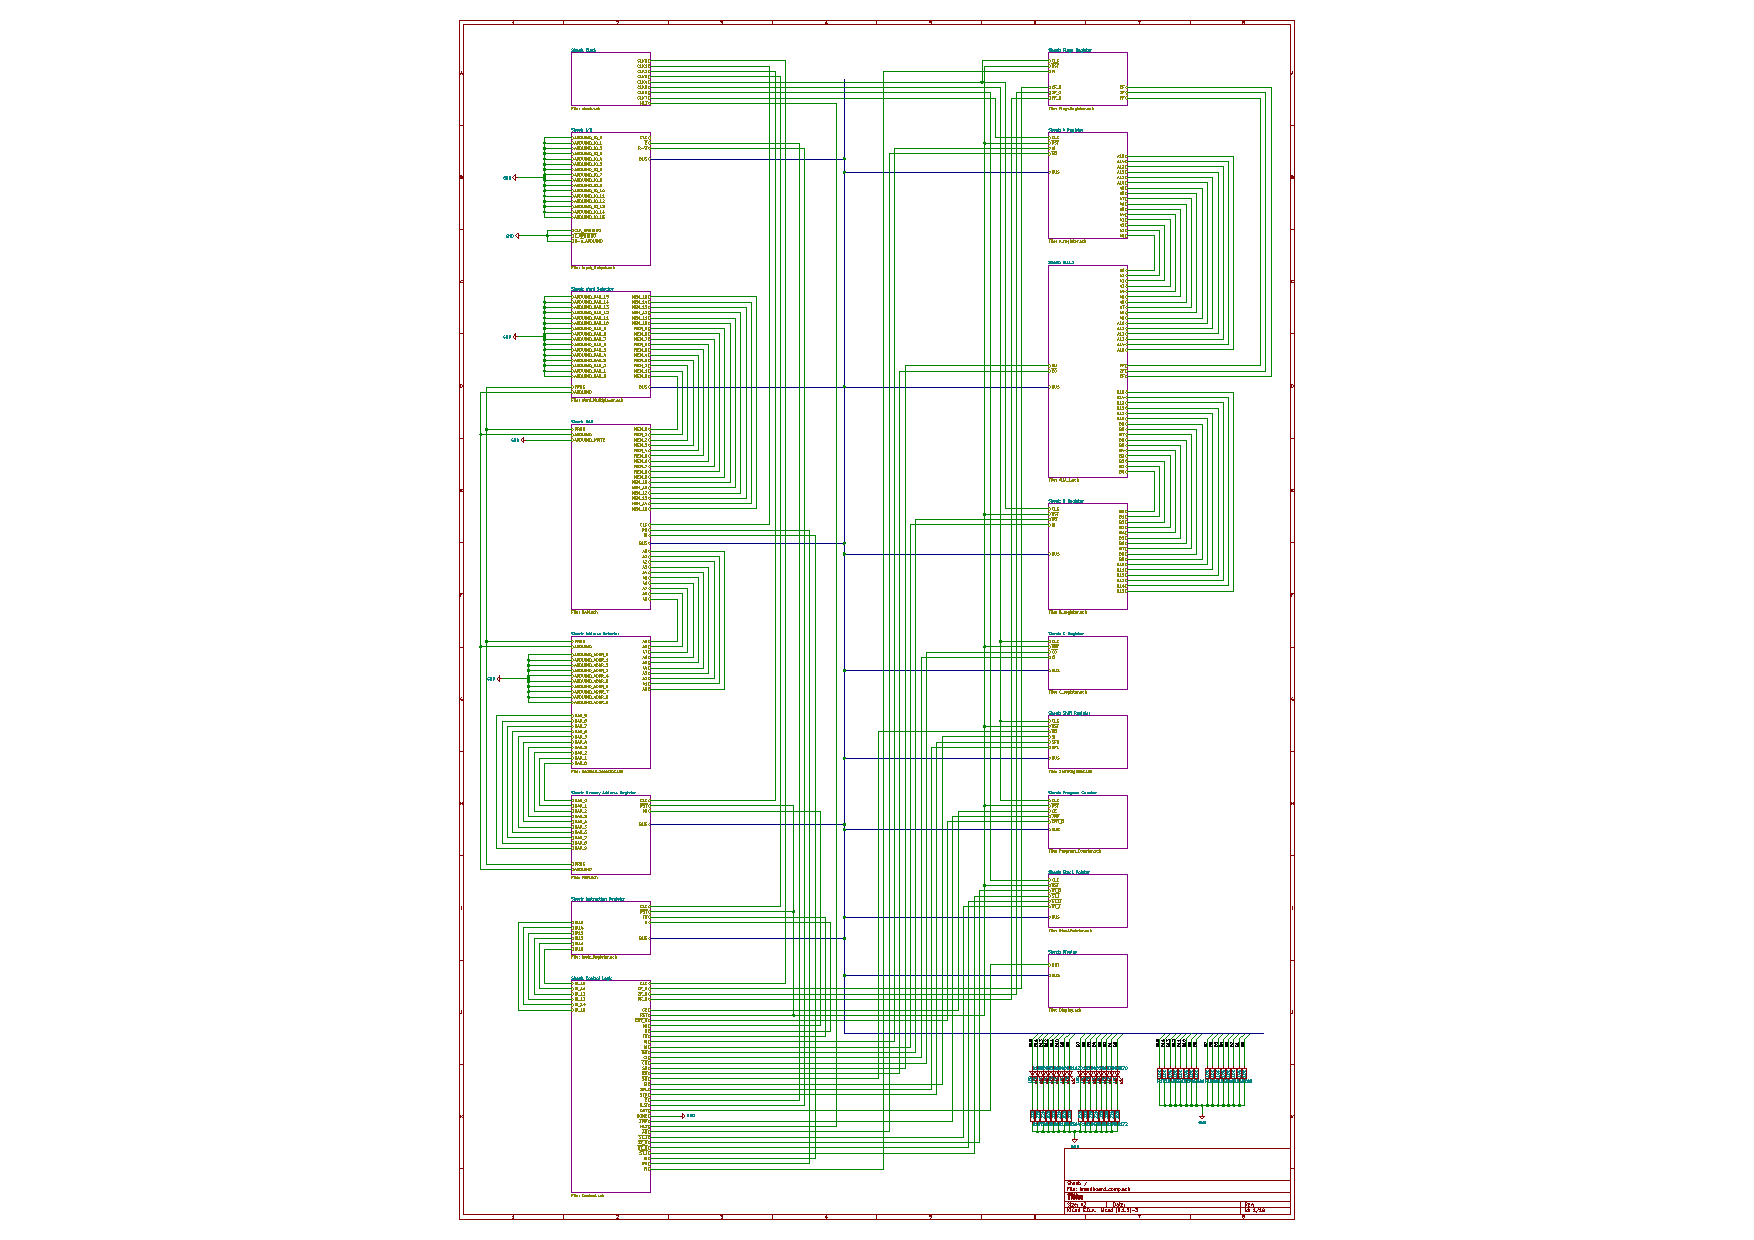
\includepdf[page={1}]{./pdf/kicad}
\clearpage

\paragraph{Clock} \ref{clock}
The clock module is very similar to the clock designed and built by Ben Eater \cite{eater2020clock}. It uses \emph{555 timers}
\cite{555} to generate a square wave which acts as the clock for the system. The \emph{555} is presented in all three most commonly
used configurations:
\begin{itemize}
  \item \emph{Astable: } it oscillates between to states (This 555 generates the main clock)
  \item \emph{Monostable: } it always ~~settles down`` to one state after a short period of time (used for the manual push-button
  clock mode)
  \item \emph{Bistable: } it has two states between which it can toggle (used for the toggle switch which goes from automatic to
  manual mode)
\end{itemize}
The clock-pulse generating \emph{555} is connected to a variable resistor which can be adjusted to increase or decrease the
frequency accordingly. A simple combinatorial circuit is used to select the appropiate clock signal and inhibit it if the \emph{HLT}
 (Halt) signal is active. The main addition to the Eater design is a \emph{74ls245 buffer} \cite{74ls245} used to amplify and
 isolate clock signals going to each module.

 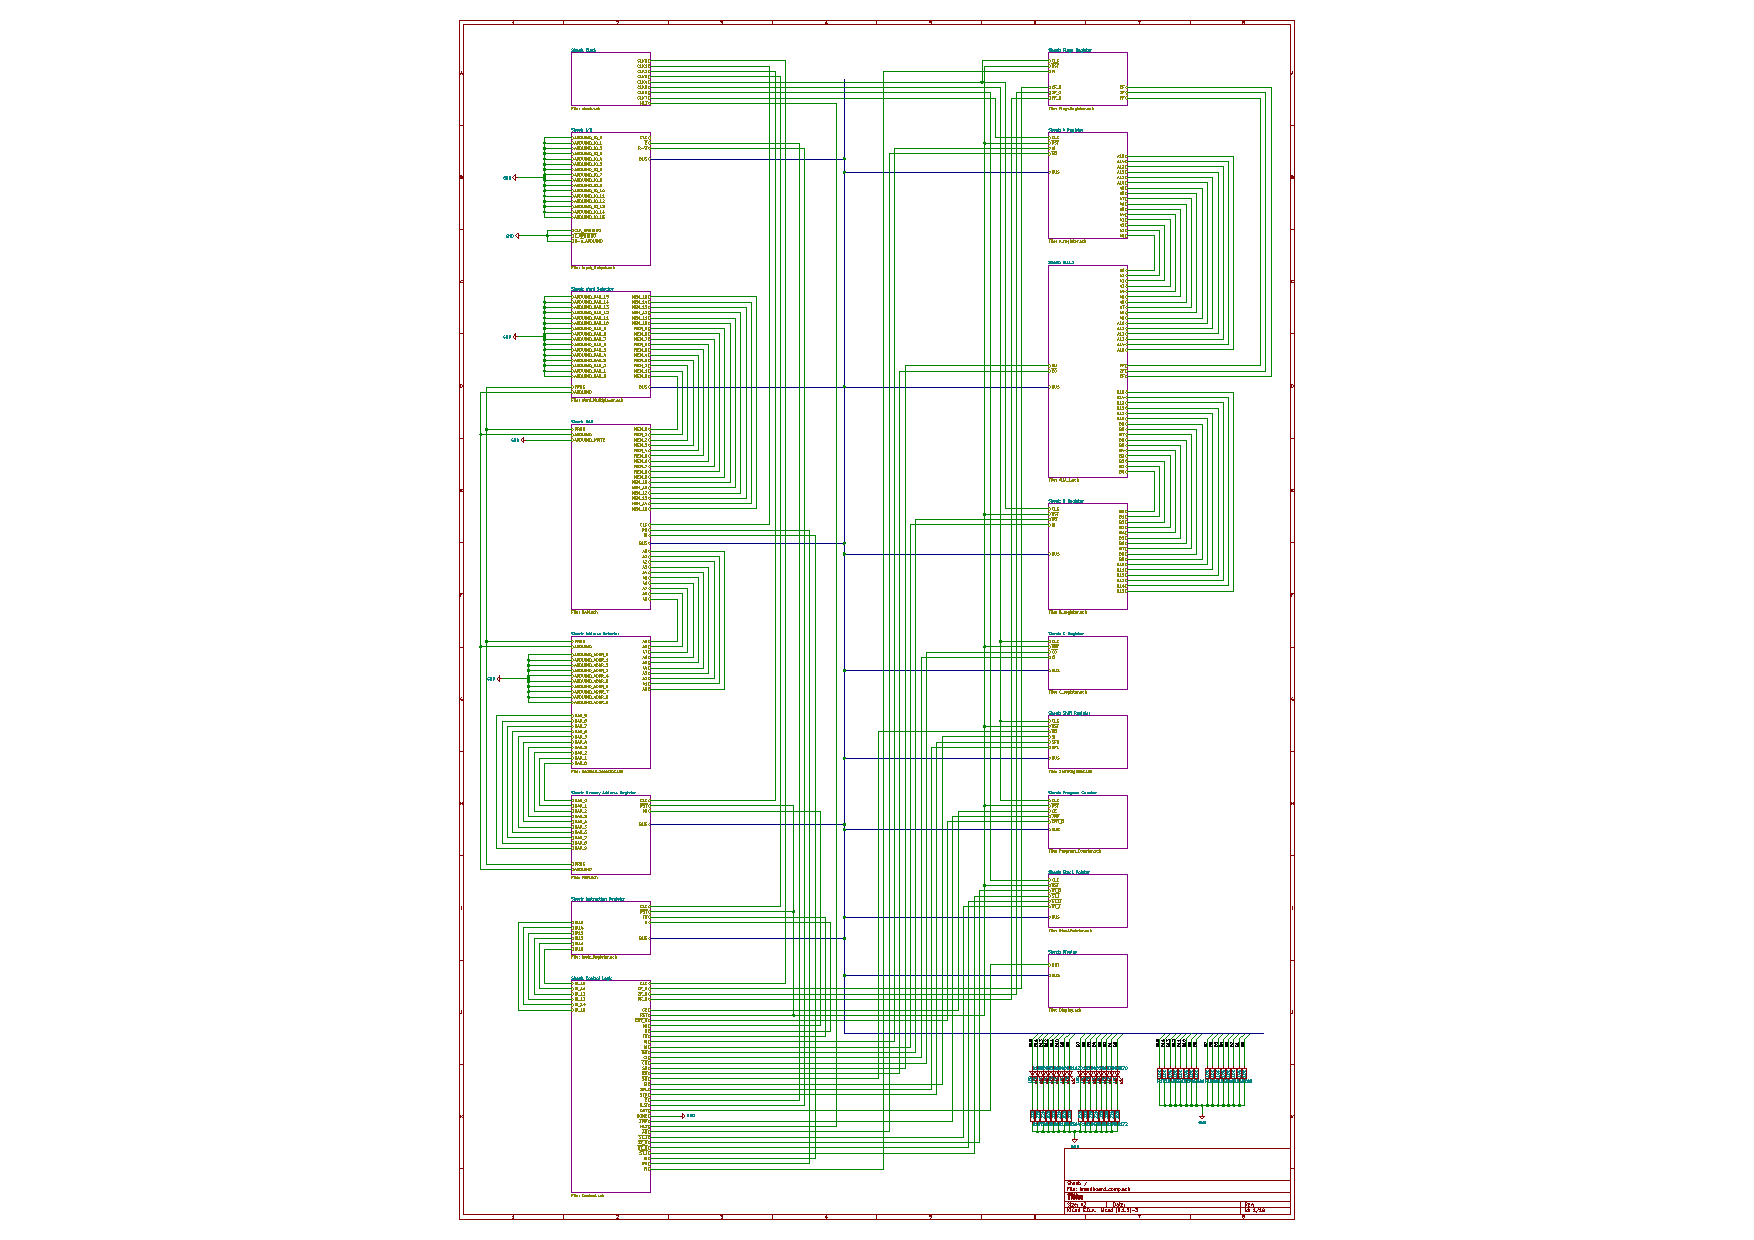
\includepdf[page={2}]{./pdf/kicad}

\paragraph{A Register} \ref{a-reg}
The A register consists of two \emph{74ls273} \cite{74ls273} 8-bit flip-flop chips and two \emph{74ls245} \cite{74ls245} buffer
interfaces to the bus. The buffers are \emph{tri-state} buffers, which means that they can pass through their input, either high or
low, or they can  disconnect their input from their output by putting themselves in a high-impedence state. This functionaility,
used across most modules which interface with the bus, is used to allow the register to assert its contents onto the bus when
reading from it (this happens when the \emph{$\overline{AO}$} signal is taken low). Writing to the register is handled by
ANDing together the \emph{AI} signal with the clock pulse. The contents of the A, which can be foud on the \emph{Q} pins, are
connected directly to the \emph{ALU} \ref{alu}.

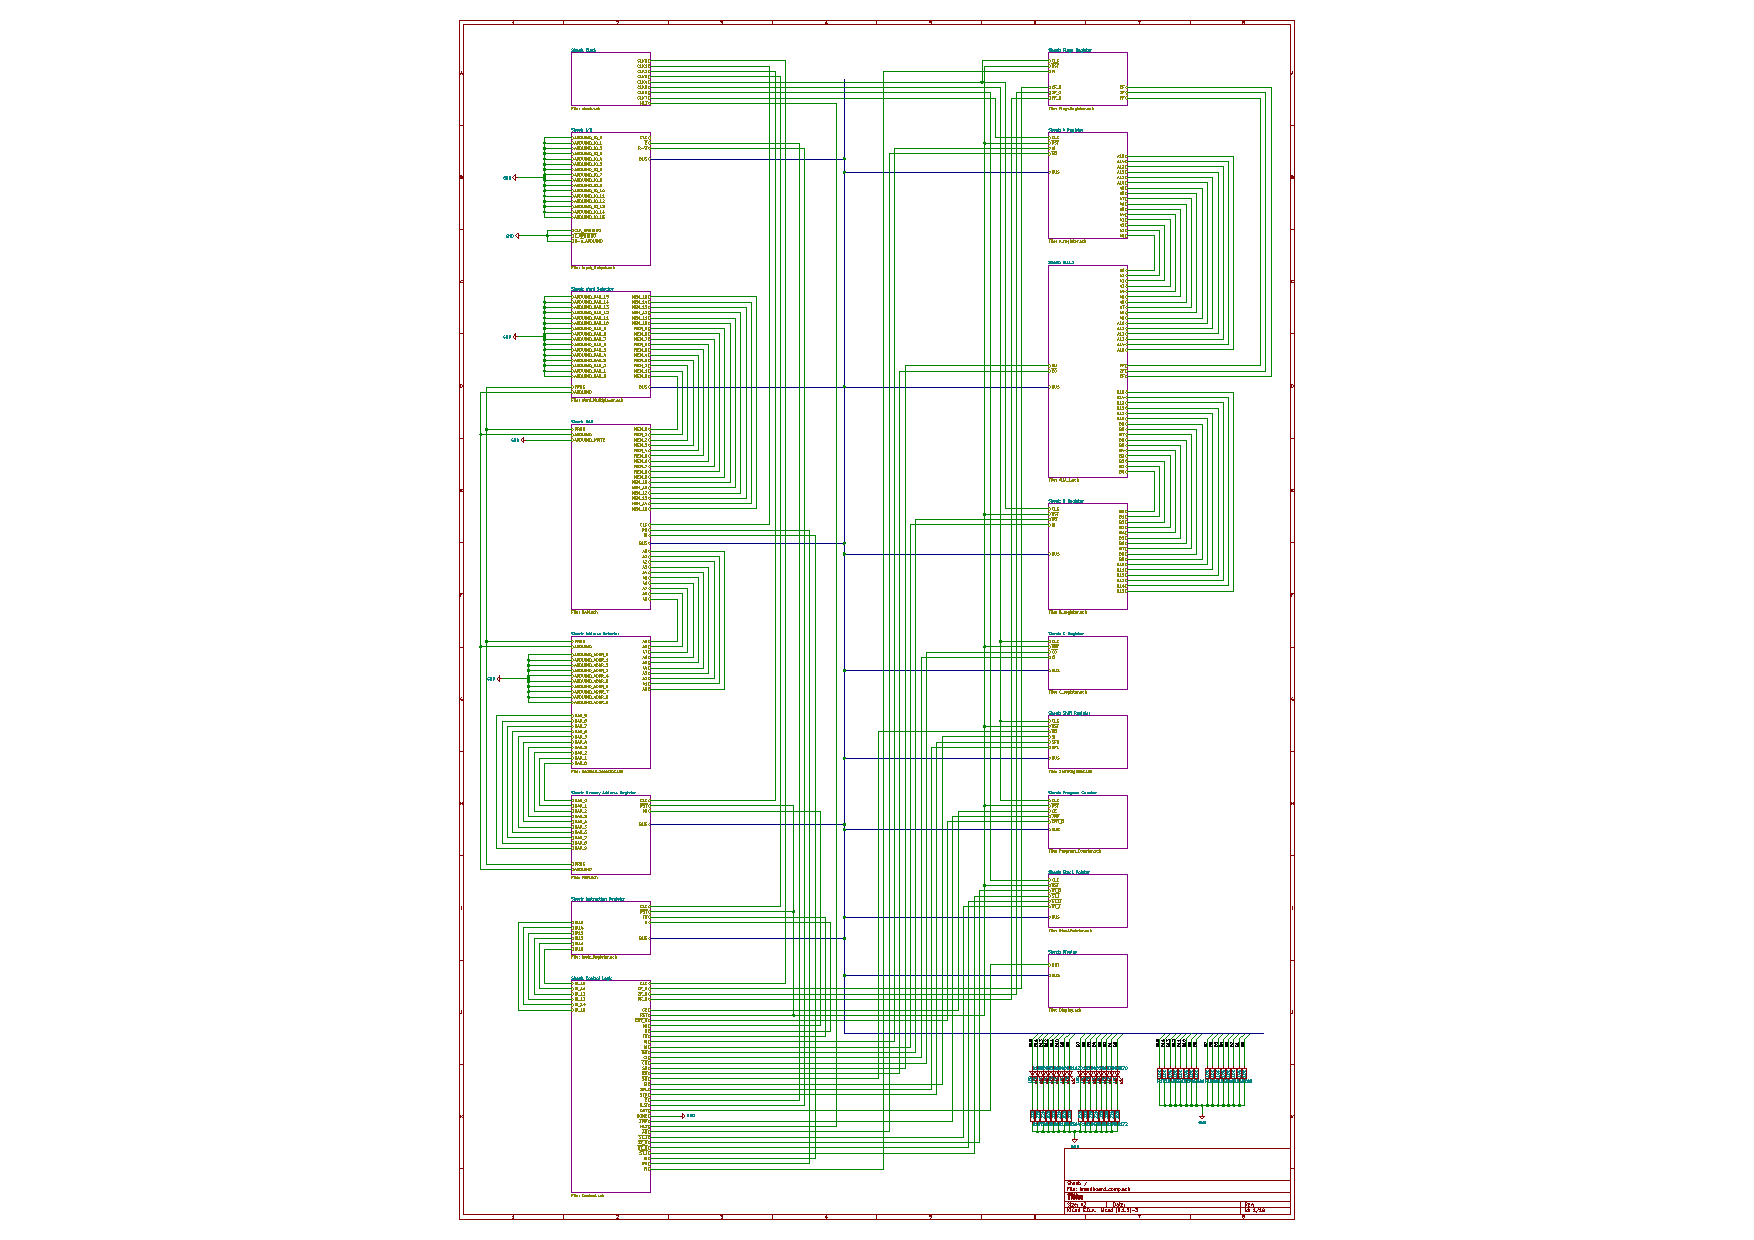
\includepdf[page={3}]{./pdf/kicad}

\paragraph{B Register} \ref{b-reg}
The B register is built essentially the same as the A register.

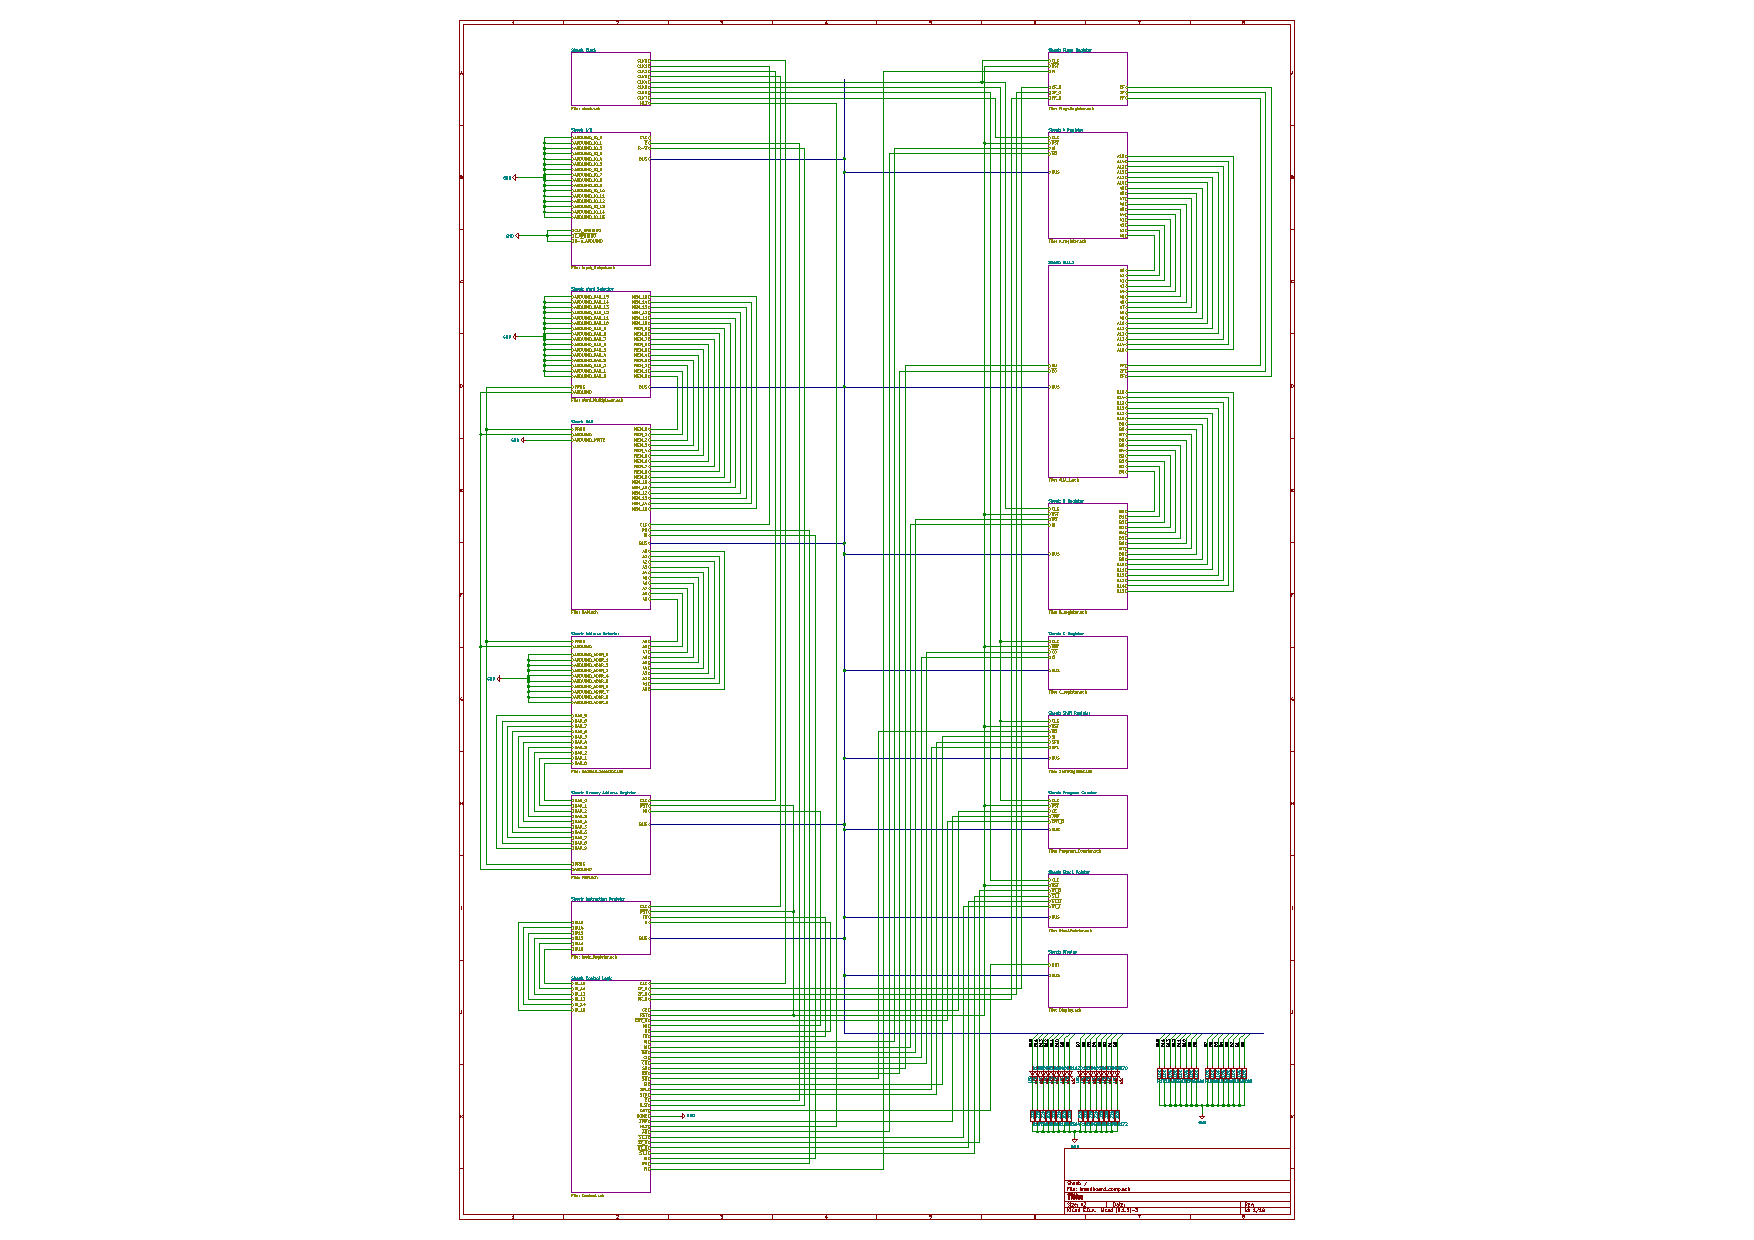
\includepdf[page={4}]{./pdf/kicad}

\paragraph{Arithmetic-Logic Unit} \ref{alu}
The \emph{ALU} has been designed around the \emph{74LS283} \cite{74ls283} chip. It contains a 4-bit binary full adder.
They can be chained together by connecting the Carry-Out of one chip to the Carry-In of the next chip. This way, by using 4
chips, a full 16-bit adder can be constructed. The A inputs are connected to the A register \ref{a-reg} and the B inputs
are conected to the B register \ref{b-reg}. The sum output is connect to two \emph{74LS245} \cite{74ls245} buffers which make the
connection to the data bus. To achieve subtraction functionality, the inputs from the B register are converted to two's complement
binary  notation, since subtracting a value equates to adding up the same negative value. To convert a positive binary value to a
two's complement negative value of the same magnitude, all 16 bits have to be flipped and then 1 has to be added to the number.
Flipping the bits is accomplished using the \emph{74LS86} \cite{74ls86} , which provides four independet XOR (exclusive or) gates.
By XORing each bit of the bit register with the value of the \emph{SU} control signal, each bit will just pass through the gate
if \emph{SU} is low and it will be flipped if \emph{SU} is high. Besides this, \emph{SU} is also connected directly to the Carry-
In Input of the first \emph{74LS283} full adder chip, to artificially add one to the final sum, representing the one which needs
to be added in for the two's complement form of the B register contents. \\
The \emph{ALU} also has three \emph{flag signals} which go out to the \emph{Flags Register} \ref{flags}. These are the \emph{Parity
Flag (PF)}, which represents the state of the lowest-significand bit of the sum, the \emph{Zero Flag (ZF)}, which is high if the
sum is 0 and low otherwise, and the \emph{Carry FLag (CF)}, which is set if the sum inside the \emph{ALU} cannot be expressed
within 16 bits. These flags can be used to make branching decisions based on the result of a calculation. The \emph{Carry Flag} and
\emph{Paritiy Flag} are straight-forward to obtain. The \emph{Carry Flag} is the Carry-Out pin of the most-significand adder
circuit. The \emph{Parity Flag} is the least significand sum pin of the least significand adder circuit. To calculate the
\emph{Zero Flag}, \emph{NOR} (inverted or) gates are employed on each pair of two sum bits. These gate can be found on the
\emph{74LS02} \cite{74ls02} chips. If any of the sum bits goes high, then the output of at least one \emph{NOR} gate will go low.
Subsequently, all \emph{NOR} outputs are ANDed together using successive \emph{AND} gates found on \emph{74LS08} \cite{74ls08}
chips. By using the and operator, if any one of the \emph{NOR} gates goes low, then the final output, which is the \emph{Zero Flag},
will go low. The only case where the \emph{Zero Flag} will go high is if all sum bits are 0.

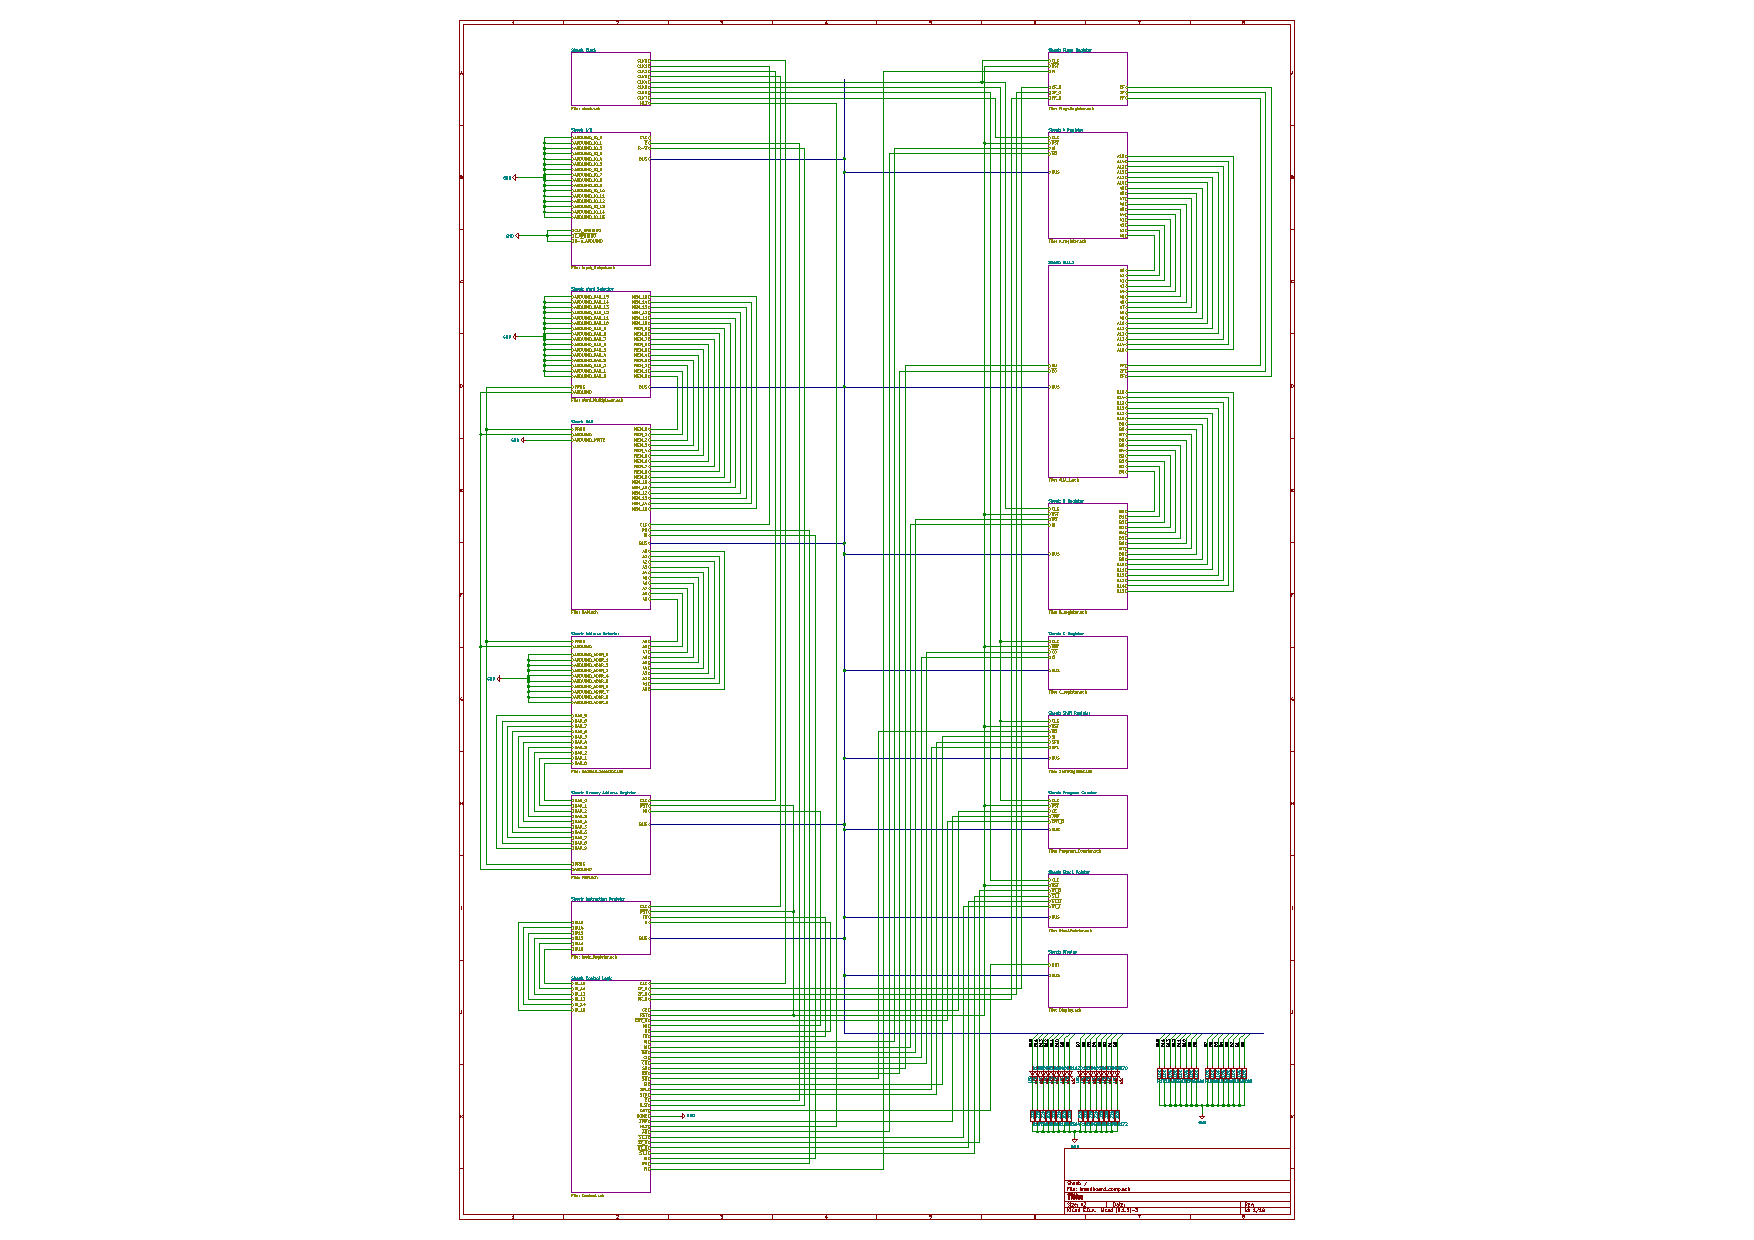
\includepdf[page={5}]{./pdf/kicad}

\paragraph{Flags Register} \ref{flags}
The Flags register consists of just one \emph{74LS273} \cite{74ls273} and some simple logic to handle the selective reads.
Allthough it is inneficient to use an 8-bit register to store only three bits, this design decision has been made because
the \emph{74ls273} is used in many other modeuls of the system and to avoid having to understand how another chip works and how
to use it.

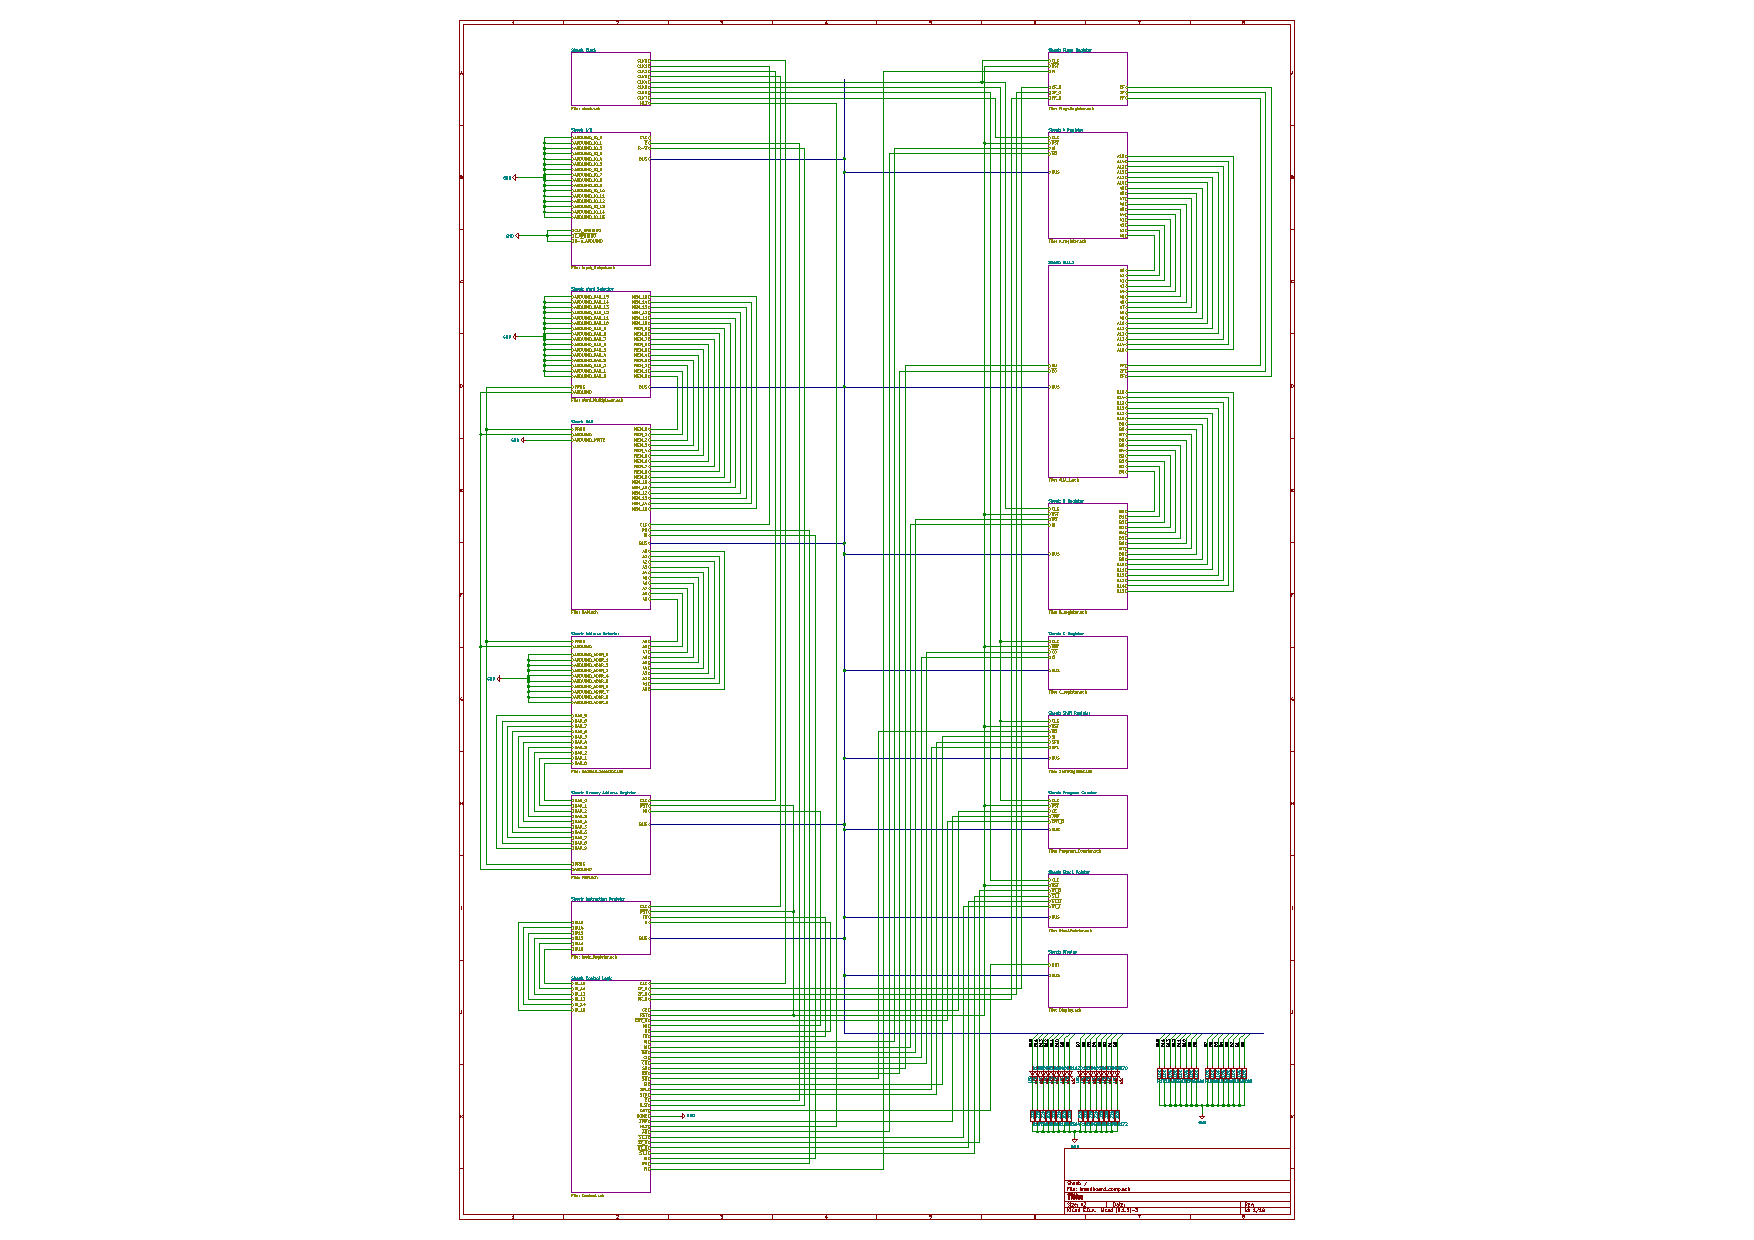
\includepdf[page={11}]{./pdf/kicad}

\paragraph{C Register} \ref{c-reg}
The C register is a general purpose 16-bit register built just like the A register \ref{a-reg} or the B register \ref{b-reg}.

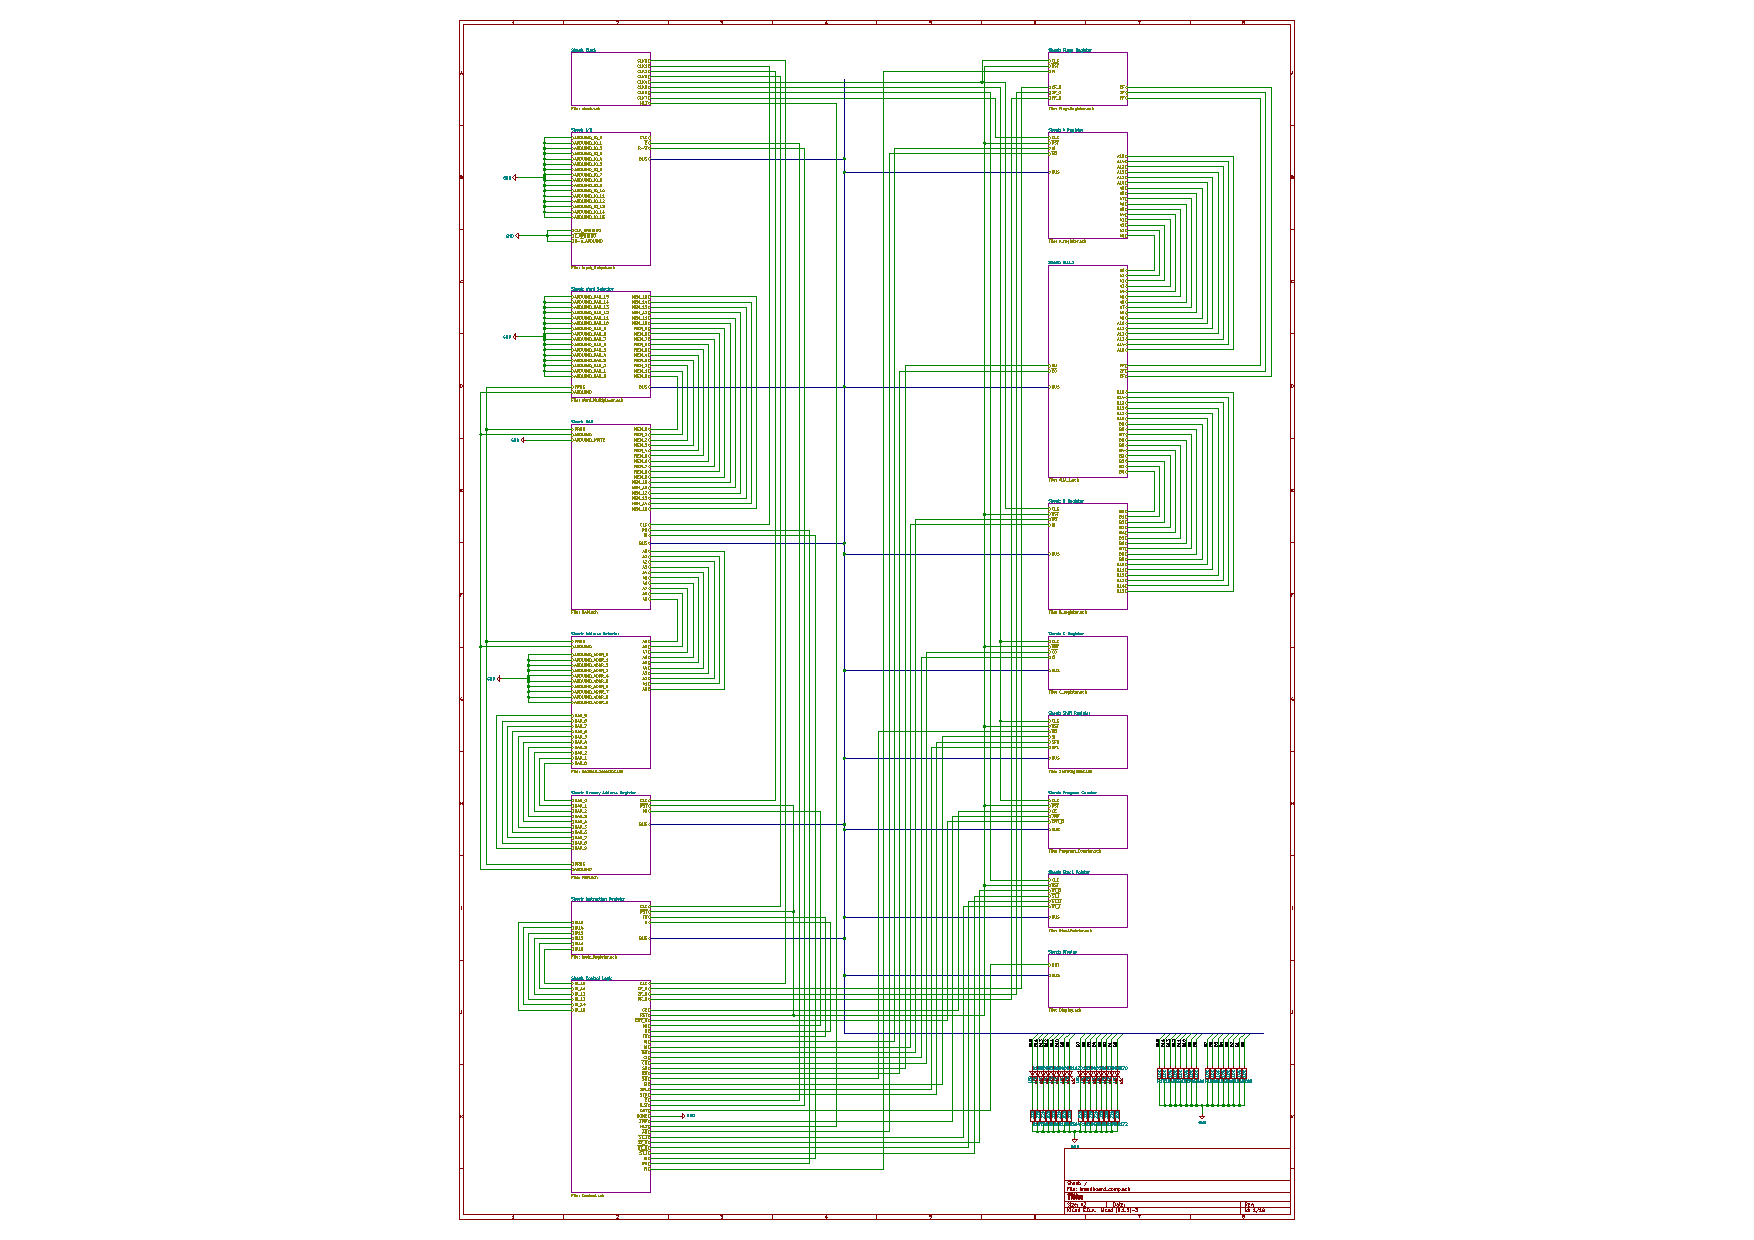
\includepdf[page={7}]{./pdf/kicad}

\paragraph{Shift Register} \ref{shift-reg}
For the design of the shift register, the \emph{74LS194} \cite{74ls194} was chosen. It is a 4-bit register which implements
bit shifting in both directions. Multiple \emph{74LS194} chips can be chained together to create a larger shift register by
connecting the Serial-Left and Serial-Right inputs of one chip to the data outputs of the chips to its left and right.
The chips have two control inputs, \emph{S0} and \emph{S1}. If both inputs are low, the register will do nothing on the next clock
pulse. If S0 or S1 is high, but not both, then a shift-right or a shift-left will occur, depending on which input is high.
If both are high, then a parallel load will occur. The data outputs of each chips are connected two two \emph{74LS245}
\cite{74ls245} chips to provided the interface to the data bus. The two control inputs are fed in from a simple combinatorial
circuit which converts the three control signals, \emph{SI}, or shift register in, \emph{SFL}, or shift left and \emph{SFR}, or
shift right, into the two lines which connect directly to the register chips.

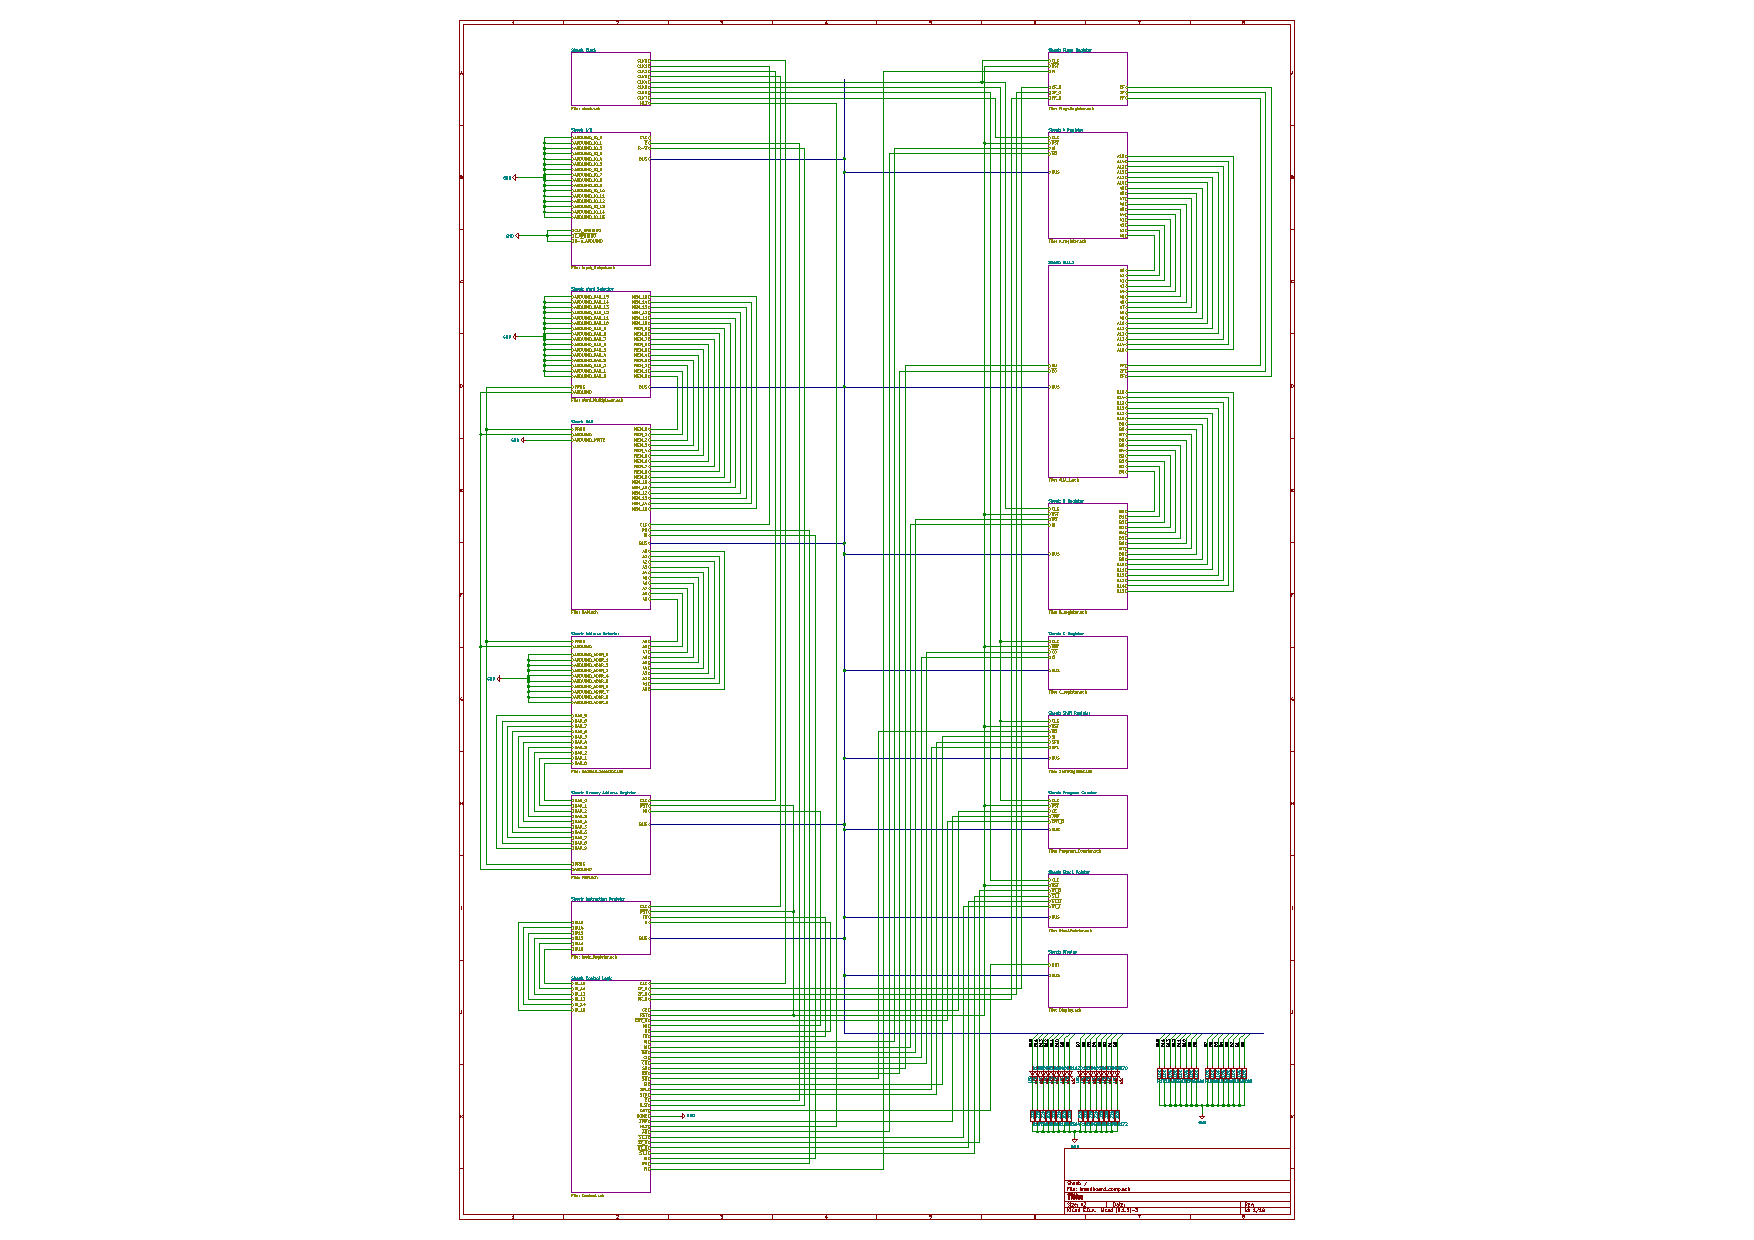
\includepdf[page={6}]{./pdf/kicad}

\paragraph{Random Access Memory (RAM)} \ref{ram}
The \emph{Random Acces Memory} module, or RAM module, poses an interesting design challenge. Thee \emph{7400} family of integrated
circuits does not include any circuits which would fulfil the 16K memory space specification previously chosen in a simple and
intuitive manner. As such, different chips had to be chosen. In the end the \emph{LY62256} 32K x 8-bit static RAM chip
\cite{ly62256} from \emph{Lynotek Inc.} and stocked by \cite{farnell} was selected. This chip was chosen because it provides
a sufficiently large address space as well as simple control inputs. Since the chips are not part of the standard symbol library,
a symbol had to be created for the \emph{LY62256} chips in the Symbol Editor. The chips have 15 address lines, too many for the
16-bit breadboard computer. This is not an issue though, as the extra lines, \emph{A10} through \emph{A14}, can be tied to logic
0 and ignored. \\
One chip stores one byte of data at any given address, so two chips were needed to adequately cover the entire 16K memory array.
Since the chips use the same pins for both data reads and writes, two sets of two \emph{74LS245} buffers \cite{74ls245}. In this
configuration, the data pins of each RAM chip are locked between two buffer chips and is, as such, effectivley isolated from the
rest of the computer. If reads a read operation is requested, the data bus facing buffers will activate and allow the data pins of
the RAM chips to drive the bus. If a write operation is requested, the word selector facing buffers will activate and allow data to
flow from the word selector to the RAM chip data pins. Besides this, some simple combinatorial logic is used to implement a selector
for the write \emph{RI} signal based on the \emph{ARDUINO} and \emph{PROG} signals.

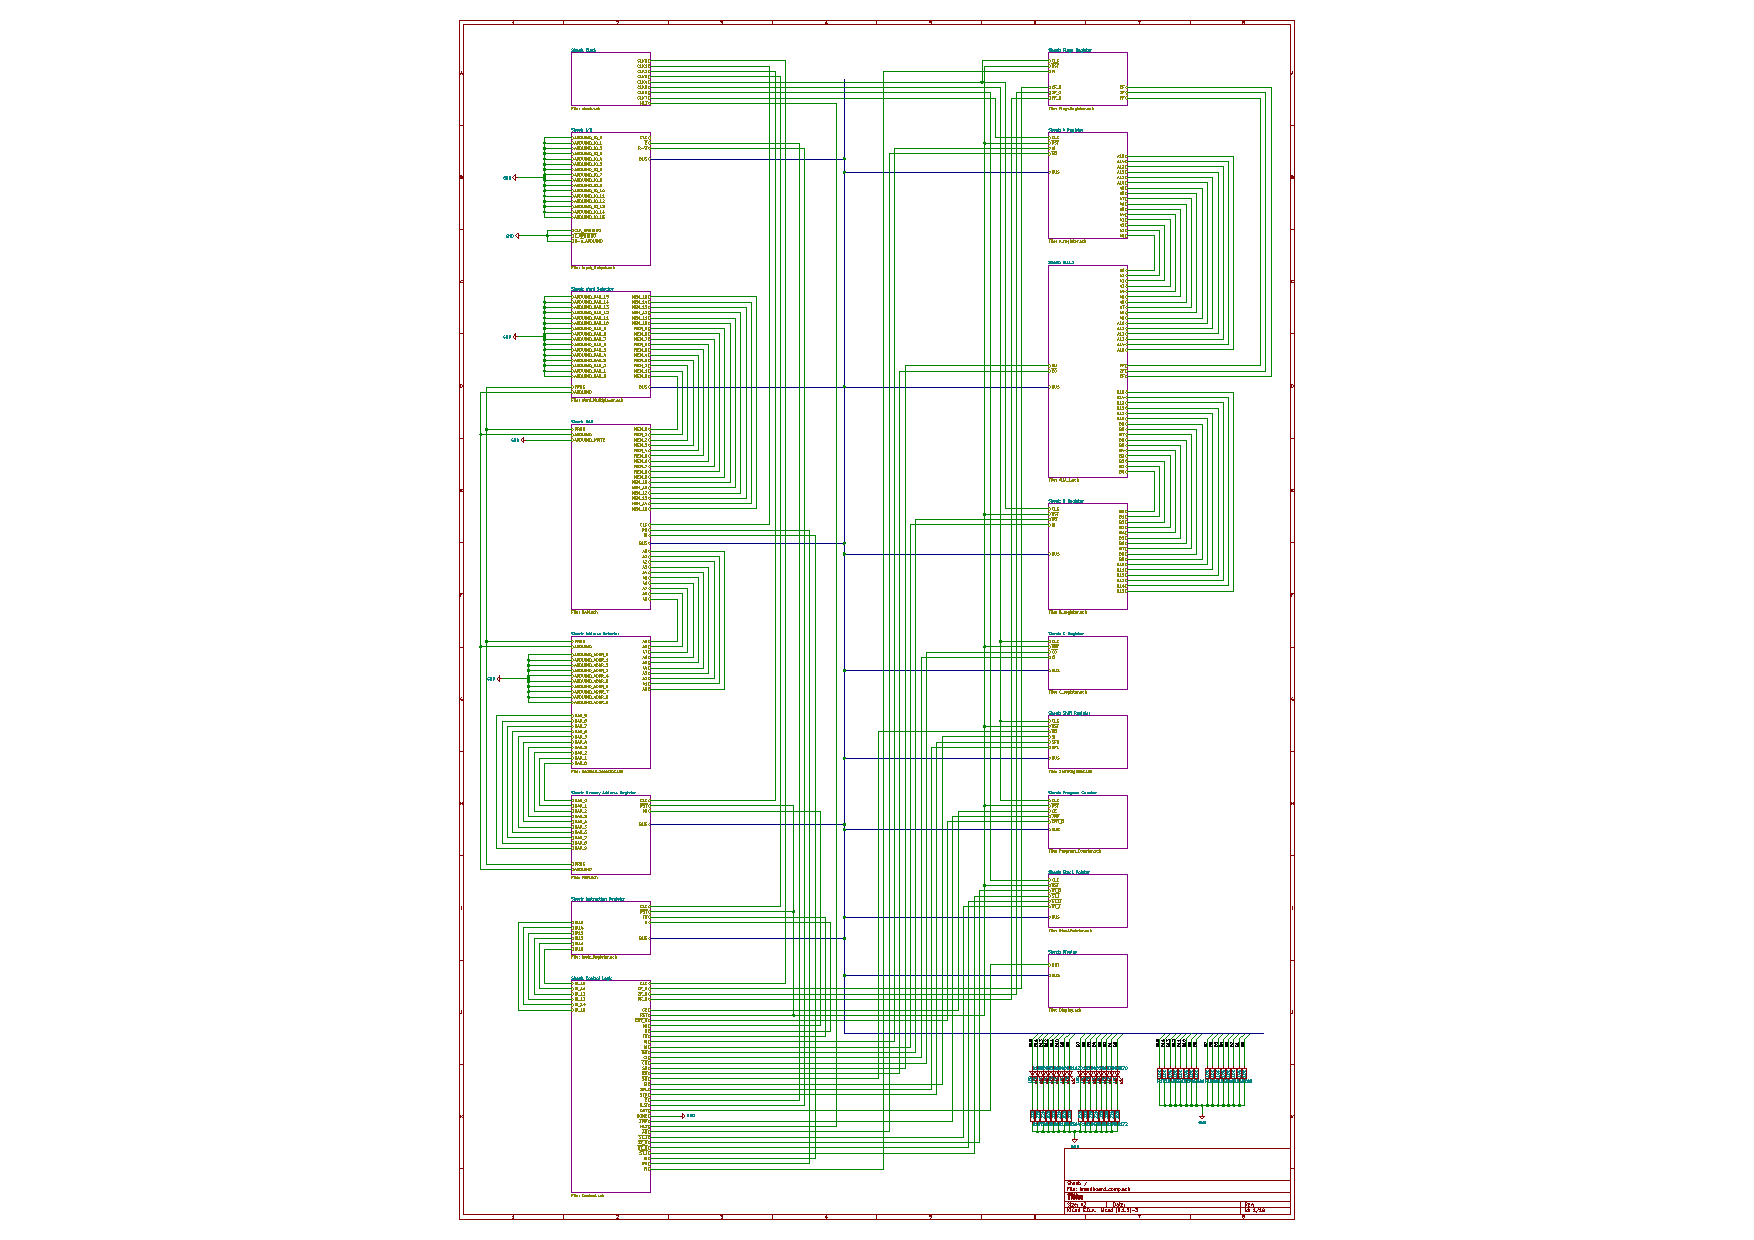
\includepdf[page={17}]{./pdf/kicad}

\paragraph{Program Counter} \ref{pc}
The centerpiece of the program counter module design is the \emph{74LS161} 4-bit binary counter \cite{74ls161}. This chips
implement most of the functionaility needed for the program counter. If the two enable signals are high, the chip will count
up in binary on the next clock pulse. If the \emph{Ripple Carry Output} pin is fed forward to the \emph{Enable T} signal of the
next counter, multiple counter can be used to create a binary counter of arbitrary length. In the case of the 16-bit breadboard
computer, to cover a 1K address space 10 bits are needed. This translates to three counters. Since the most significand two bits of
the most significand counter are not needed, the Q2 pin can be integrated into the reset circuit, so that the counter loops back
to 0 after reaching \emph{0x3FF}. Besides this, by having a parallel load pin, the \emph{74LS161}  facilitates jump functionailty,
used for programming branch and loop instructions. As usual, the bus interface is handled by two \emph{74LS245} \cite{74ls245}
chips. Since only 10 bits are connected from the counter chips to the buffers, the remaining six bits are tied low.
The control signals are decoded using simple combinatorial logic.

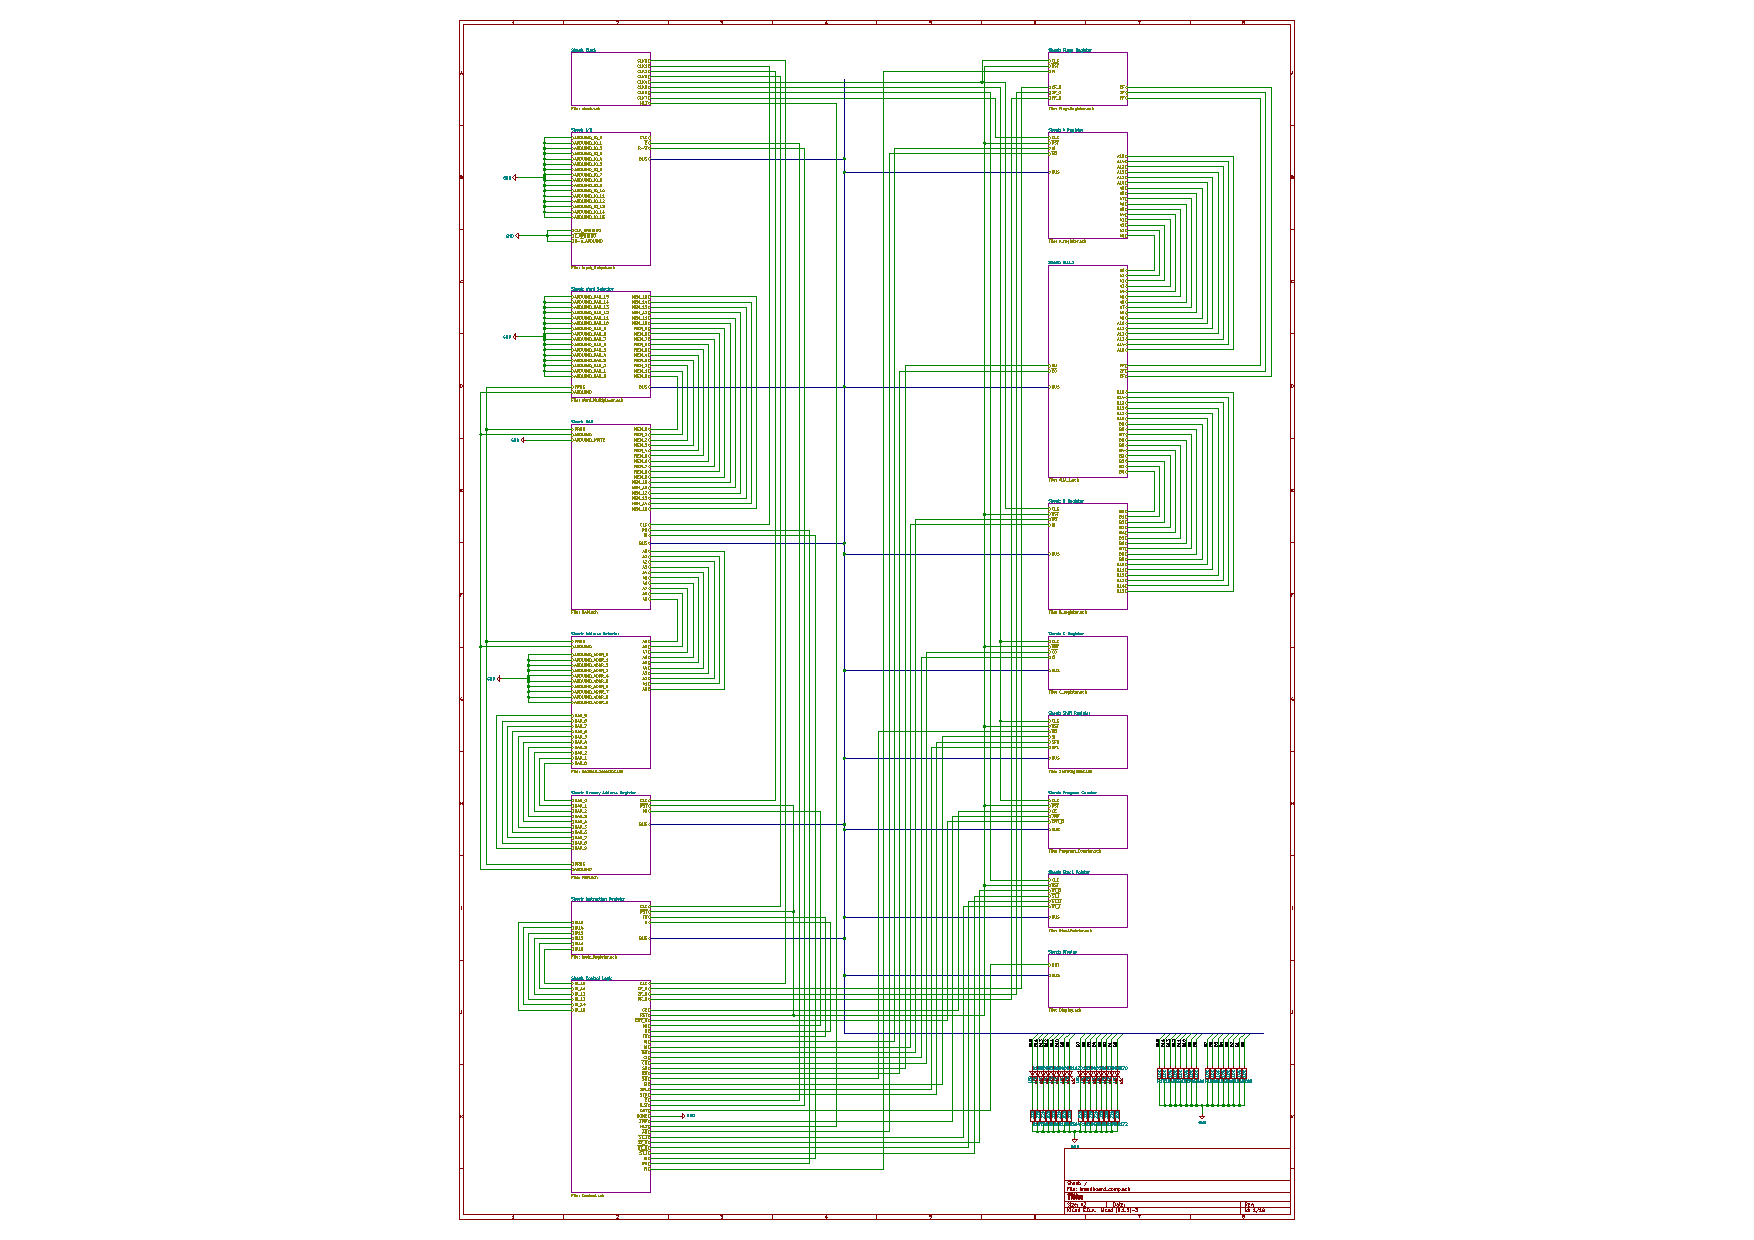
\includepdf[page={10}]{./pdf/kicad}

\paragraph{Stack Pointer} \ref{stack-pointer}
The stack is designed using a \emph{74LS169} 4-bit binary up-down counter chip \cite{74ls169}. Allthough limited,
the chip fits the specification because only a small fraction of the address space is alloted to the stack. The stack is formed
of the last 16 addresses, so only 4 bits are needed to specify them, since the remaining 6 bits are identical for all stack
addresses. The \emph{74LS169} differs from the \emph{74LS161} \cite{74ls161} used in the Program Counter \ref{pc} in the fact that
it trades in the master reset pin with the up-down pin, which controls which way the counter counts. As such, to preserve reset
functionality, a \emph{74LS157} \cite{74ls157} multiplexer chip is used. This chip selects between two sets of 4 bits based on
the state of a single control bit. This is used in the stack pointer for loading in either the lowest significant four data bus
bits, in case a stack jump is to be executed, and 4 low values, in case a reset is to be executed. This restores the missing
reset functionality. Besides this, two \emph{74LS245} \cite{74ls245}  chips are used to interface to the bus. Besides the four
bits provided by the stack pointer, the next six bits are tied to logic 1, to reflect the position of the stack address range in
the memory space. The rest are tied to logic 0. Finally, some simple gate logic manages the control signals.

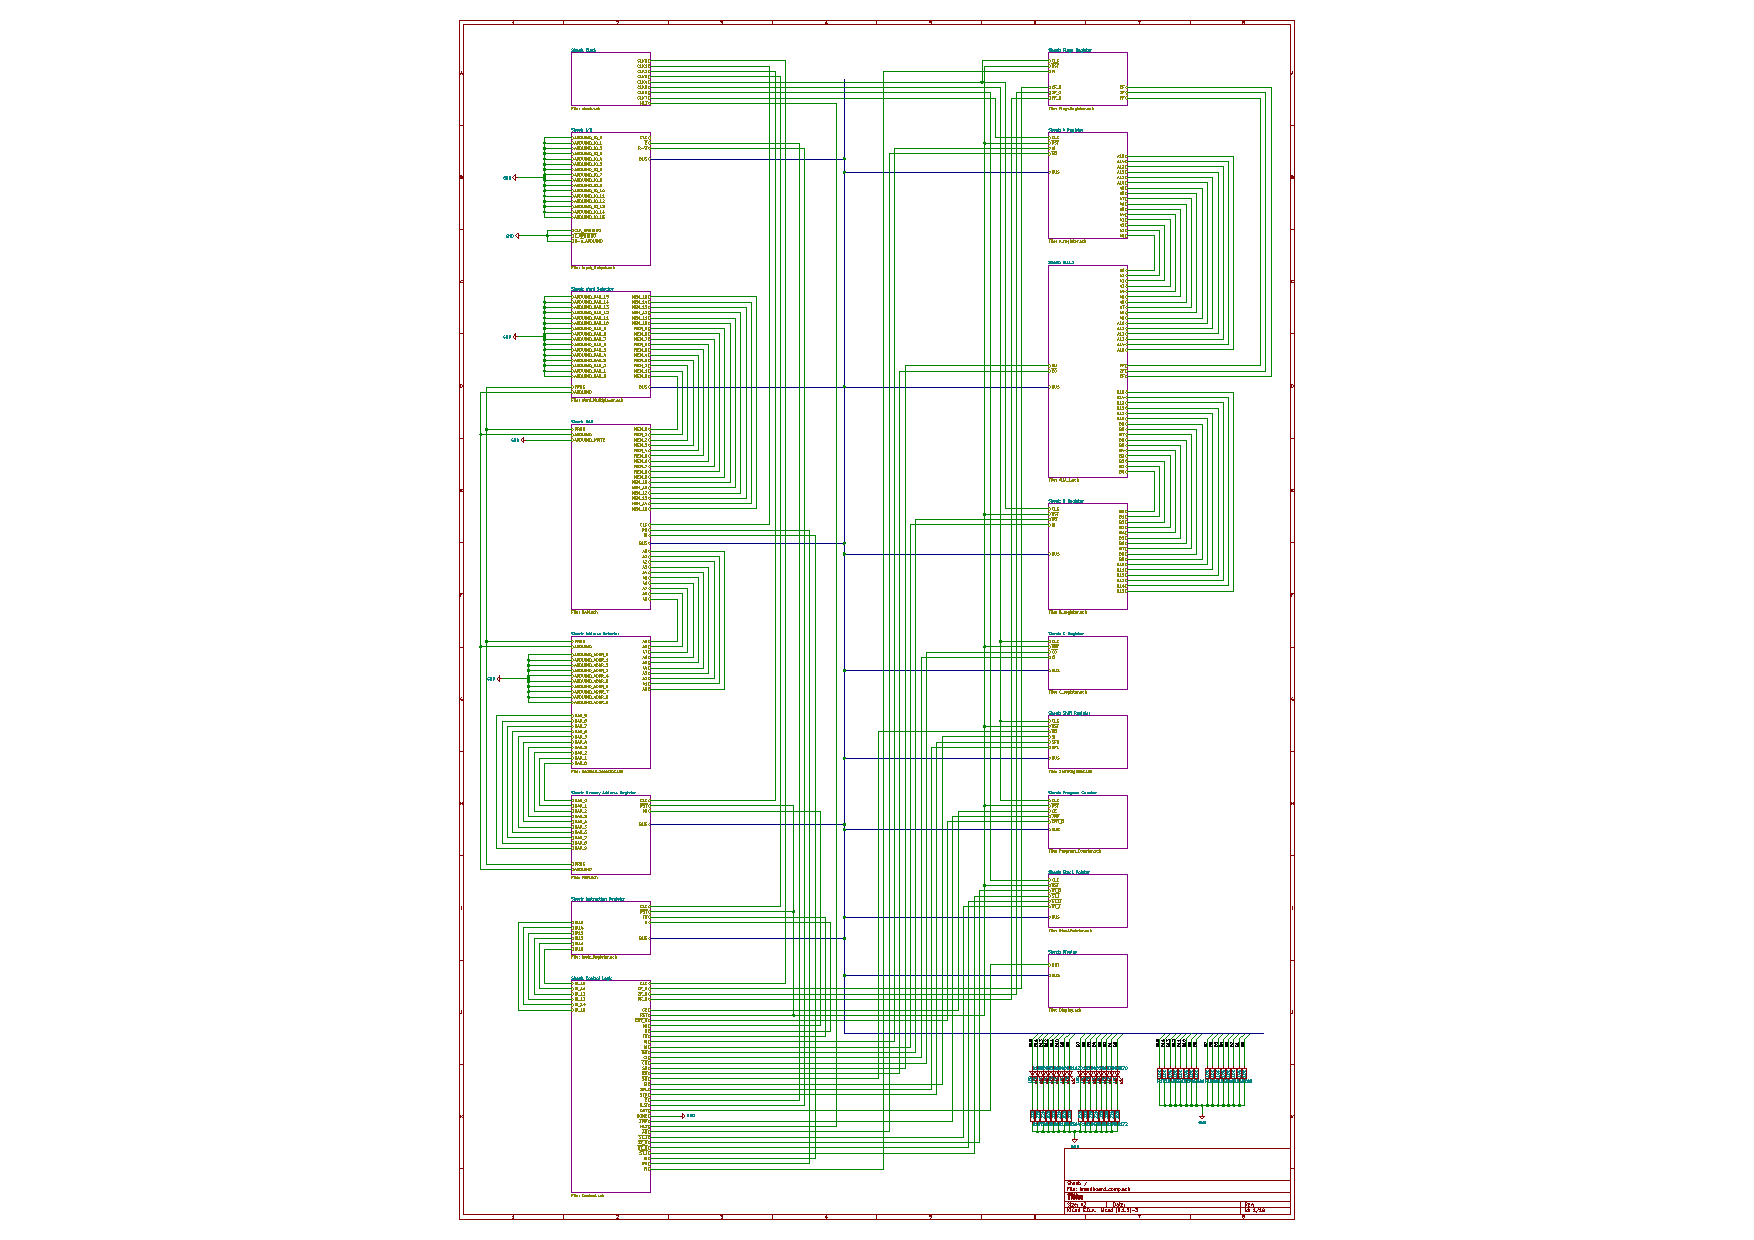
\includepdf[page={14}]{./pdf/kicad}

\paragraph{Display} \ref{display}
To fit the specification of a 16 characters by two line display, while maintaining relative simplicity, the \emph{c1602a v1.2}
\cite{c1602a} was chosen. This simple and widley popular LCD modules are easy enough to use and abstract a sizable amount of the
issues with character generation and display, so that a single person can master them in a relativley short span of time. They have
an internal character set and also allow the user to specify as small set of custom characters. To interact with the
\emph{c1602a v1.2}, a word of 9 bits is sent to the display on the rising edge of the \emph{Out} signal. The first bit
specifies wheter a command or a character is sent to the display, and the remaining byte represents the command or the character.
The display also implements functionailty which allows the main processor to read data from it, but this will be abstracted away,
as it is not part of the specification. Besides the data and \emph{Out} signal, the \emph{c1602a} requires just power connection
for the processor and backlight, as well as a variable resistor for the adjustable contrast.
Besides the display, two \emph{74LS245} buffer chips \cite{74ls245} are used to interface the display to the data bus. That being
said, only the least significand 9 data bits pass trough the buffer to the display, as that's all that is required.

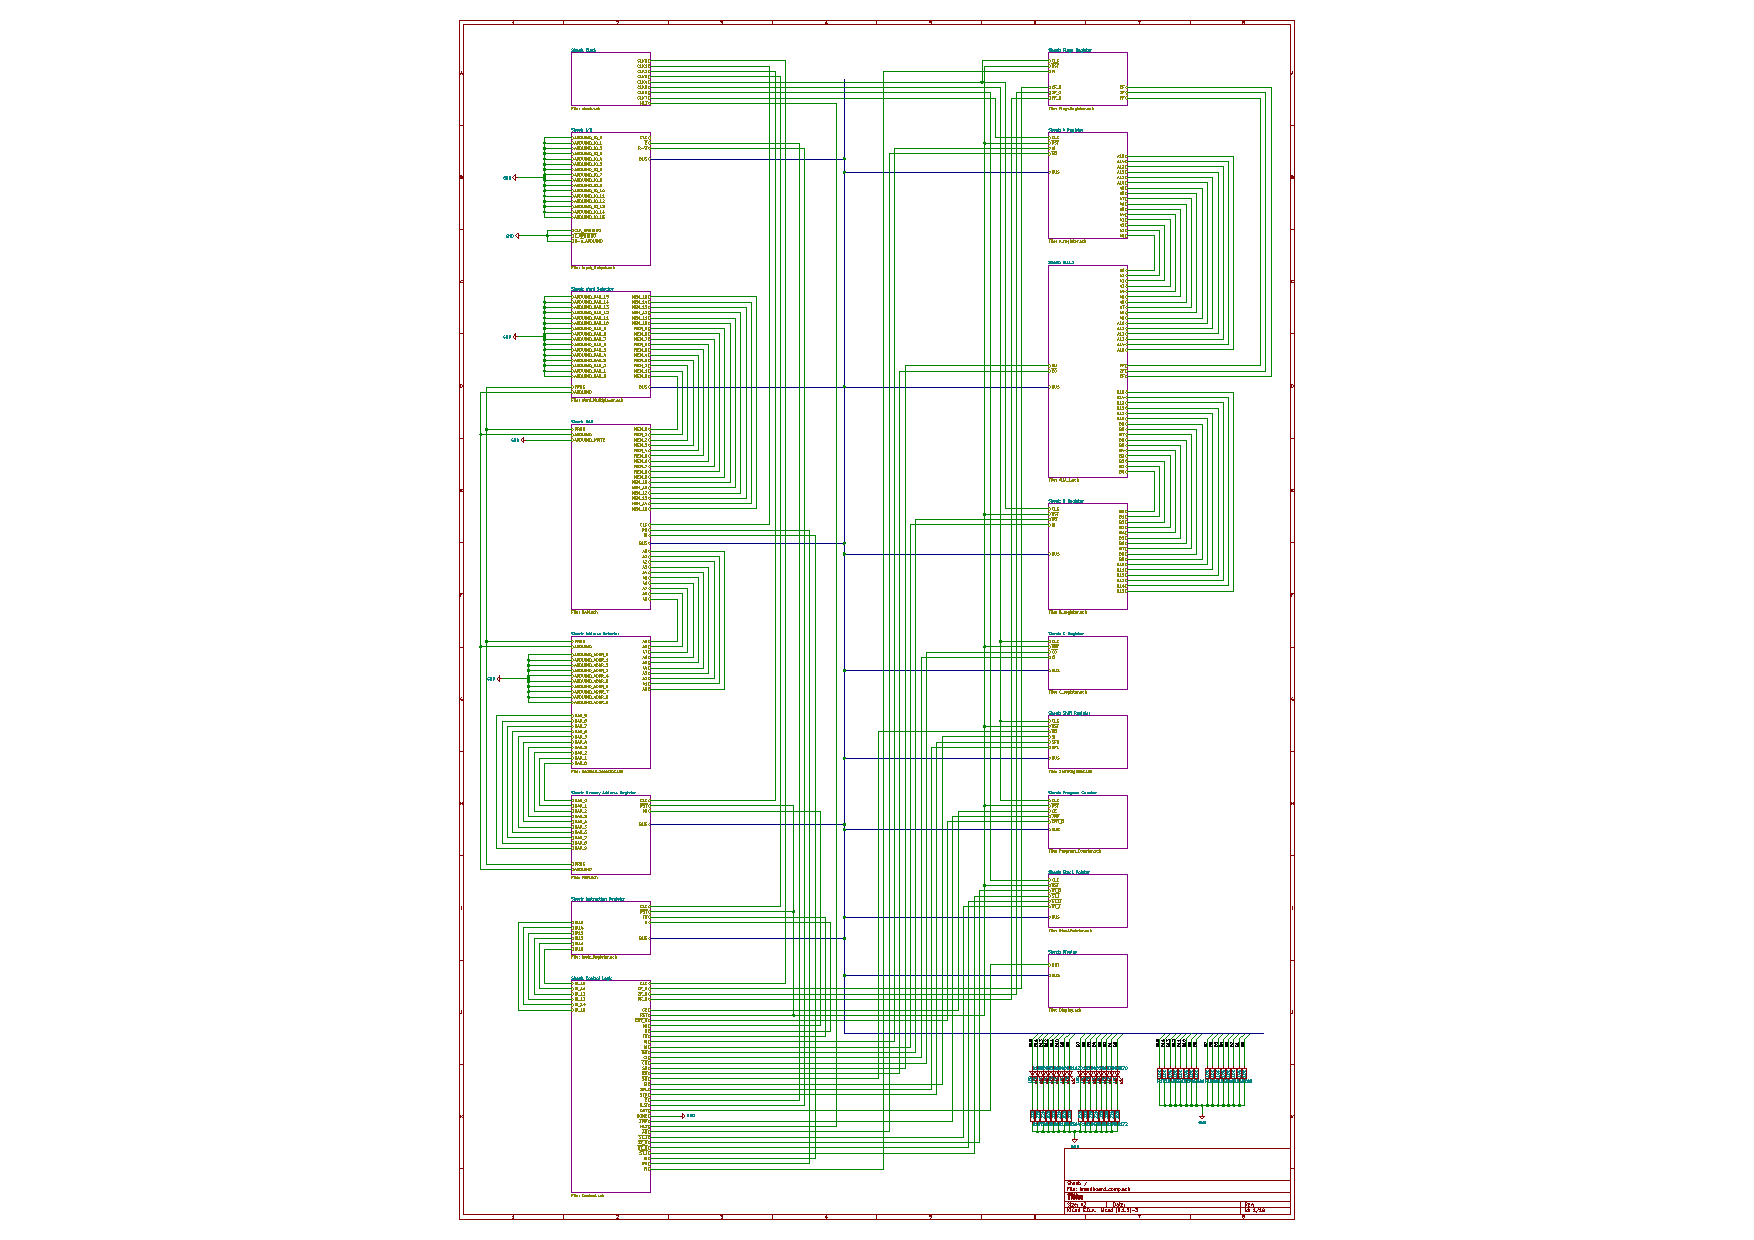
\includepdf[page={12}]{./pdf/kicad}

\paragraph{I/O} \ref{io}
The I/O module provides outside connective to an \emph{Arduino Mega} \cite{arduino2020mega}. To achieve this, two \emph{74LS245}
\cite{74ls245} buffer chips are used. When the buffers are disabled, the  Arduino and the main system are essentially
disconnected. This ensures that there is no interference when no I/O requests are issued. Furthermore, the buffers are
actually bi-directional, so by means of the \emph{Read/Write} control signal, the computer can control if data flows from
the data bus to the arduino in case of an I/O write, or the other way around in case of an I/O read. The arduino can use the
\emph{Enable} signal to trigger an interrupt and handle the I/O request and the same \emph{Read/Write} to decide what the type
of the I/O request is and handle it accordingly.

 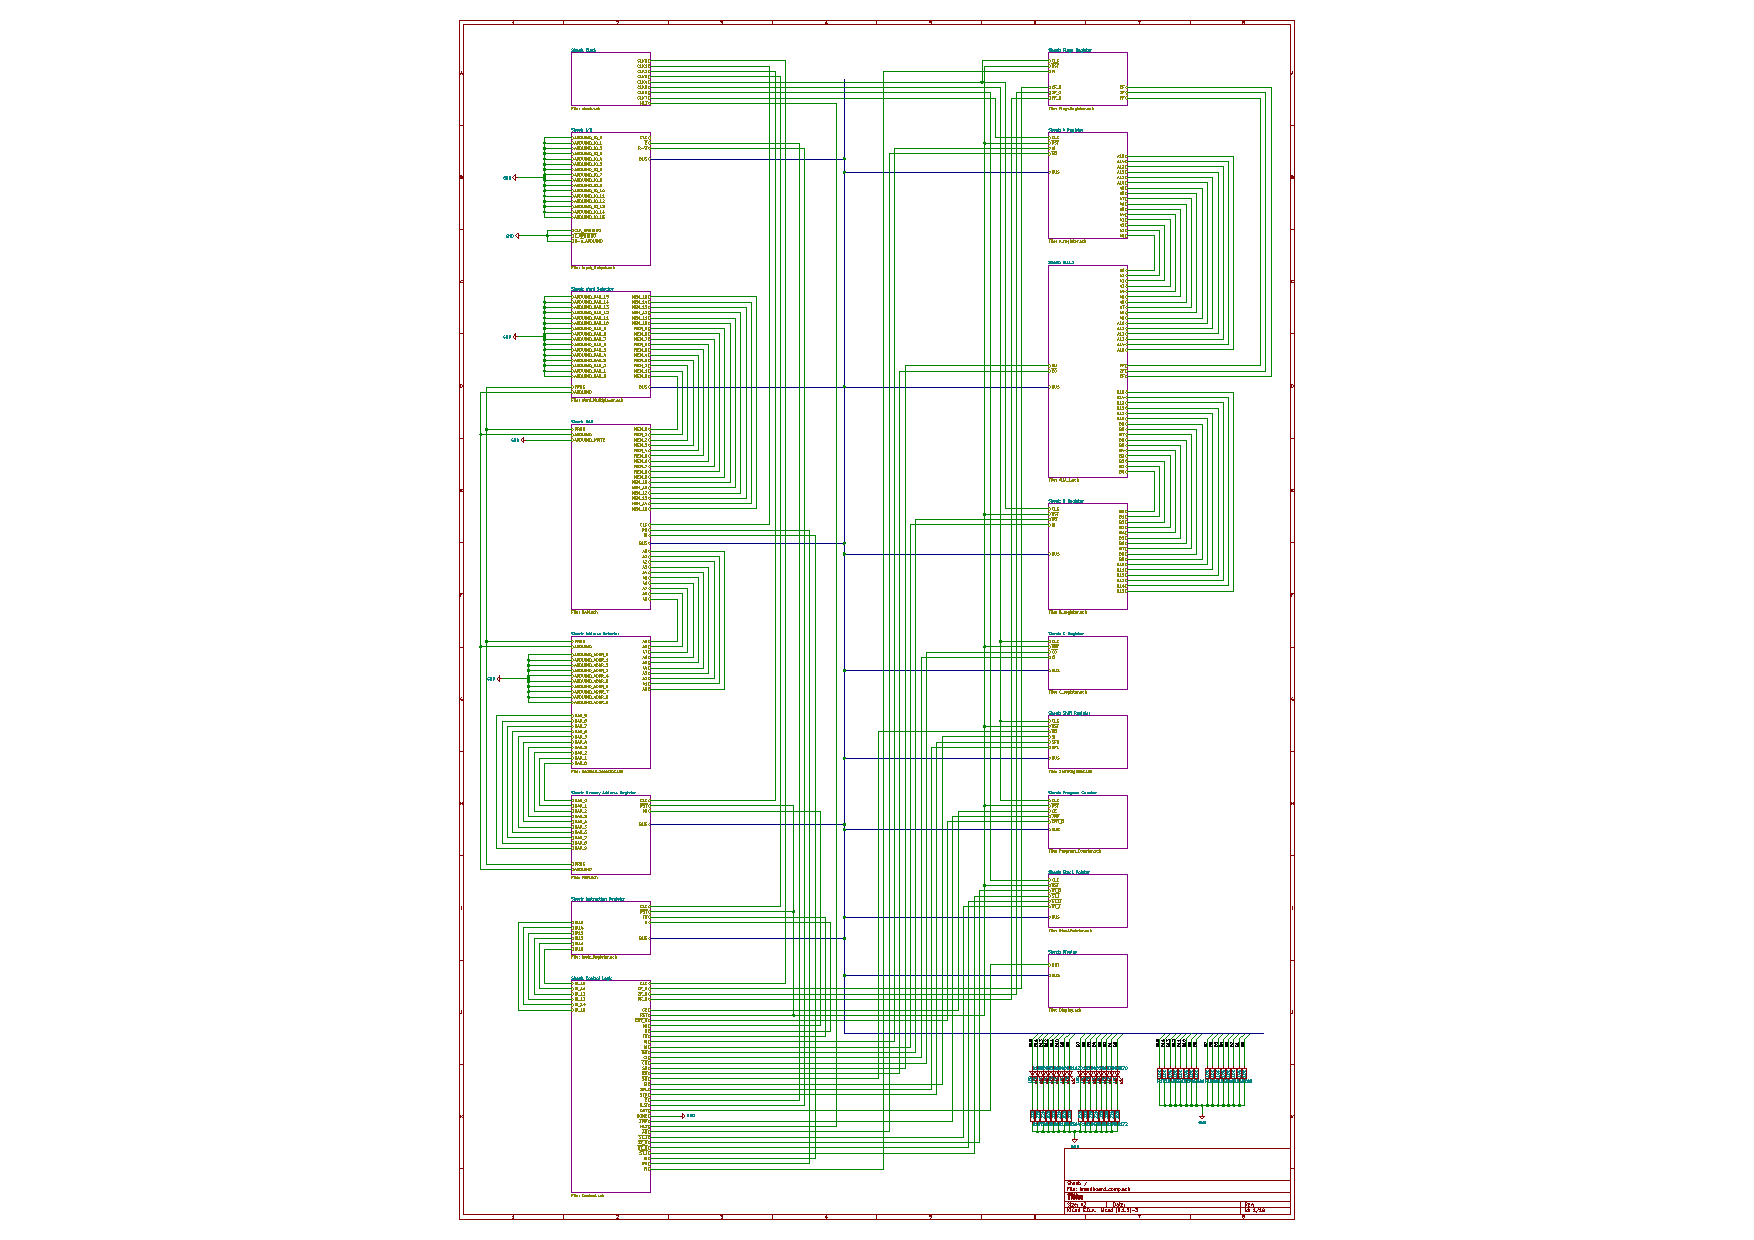
\includepdf[page={13}]{./pdf/kicad}

 \paragraph{Memory Address Register} \ref{mar}
 To design the memory address register, the same chips which was used in the A register \ref{a-reg}, the B register \ref{b-reg},
 the C register \ref{c-reg} and the flags register \ref{flags}, namely the \emph{74LS273}
  \cite{74ls273} , comes to mind. Since the memory address register will not assert its contents to the bus, there is no need for
 a data bus buffer. But, since the module is built up of few components and is placed in the vicinity of RAM \ref{ram} and the
 address selector \ref{addr-select}, it lends itself as a good location for the two toggle switches which will be used to
 set the \emph{ARDUINO} And \emph{PROG} control signals.

 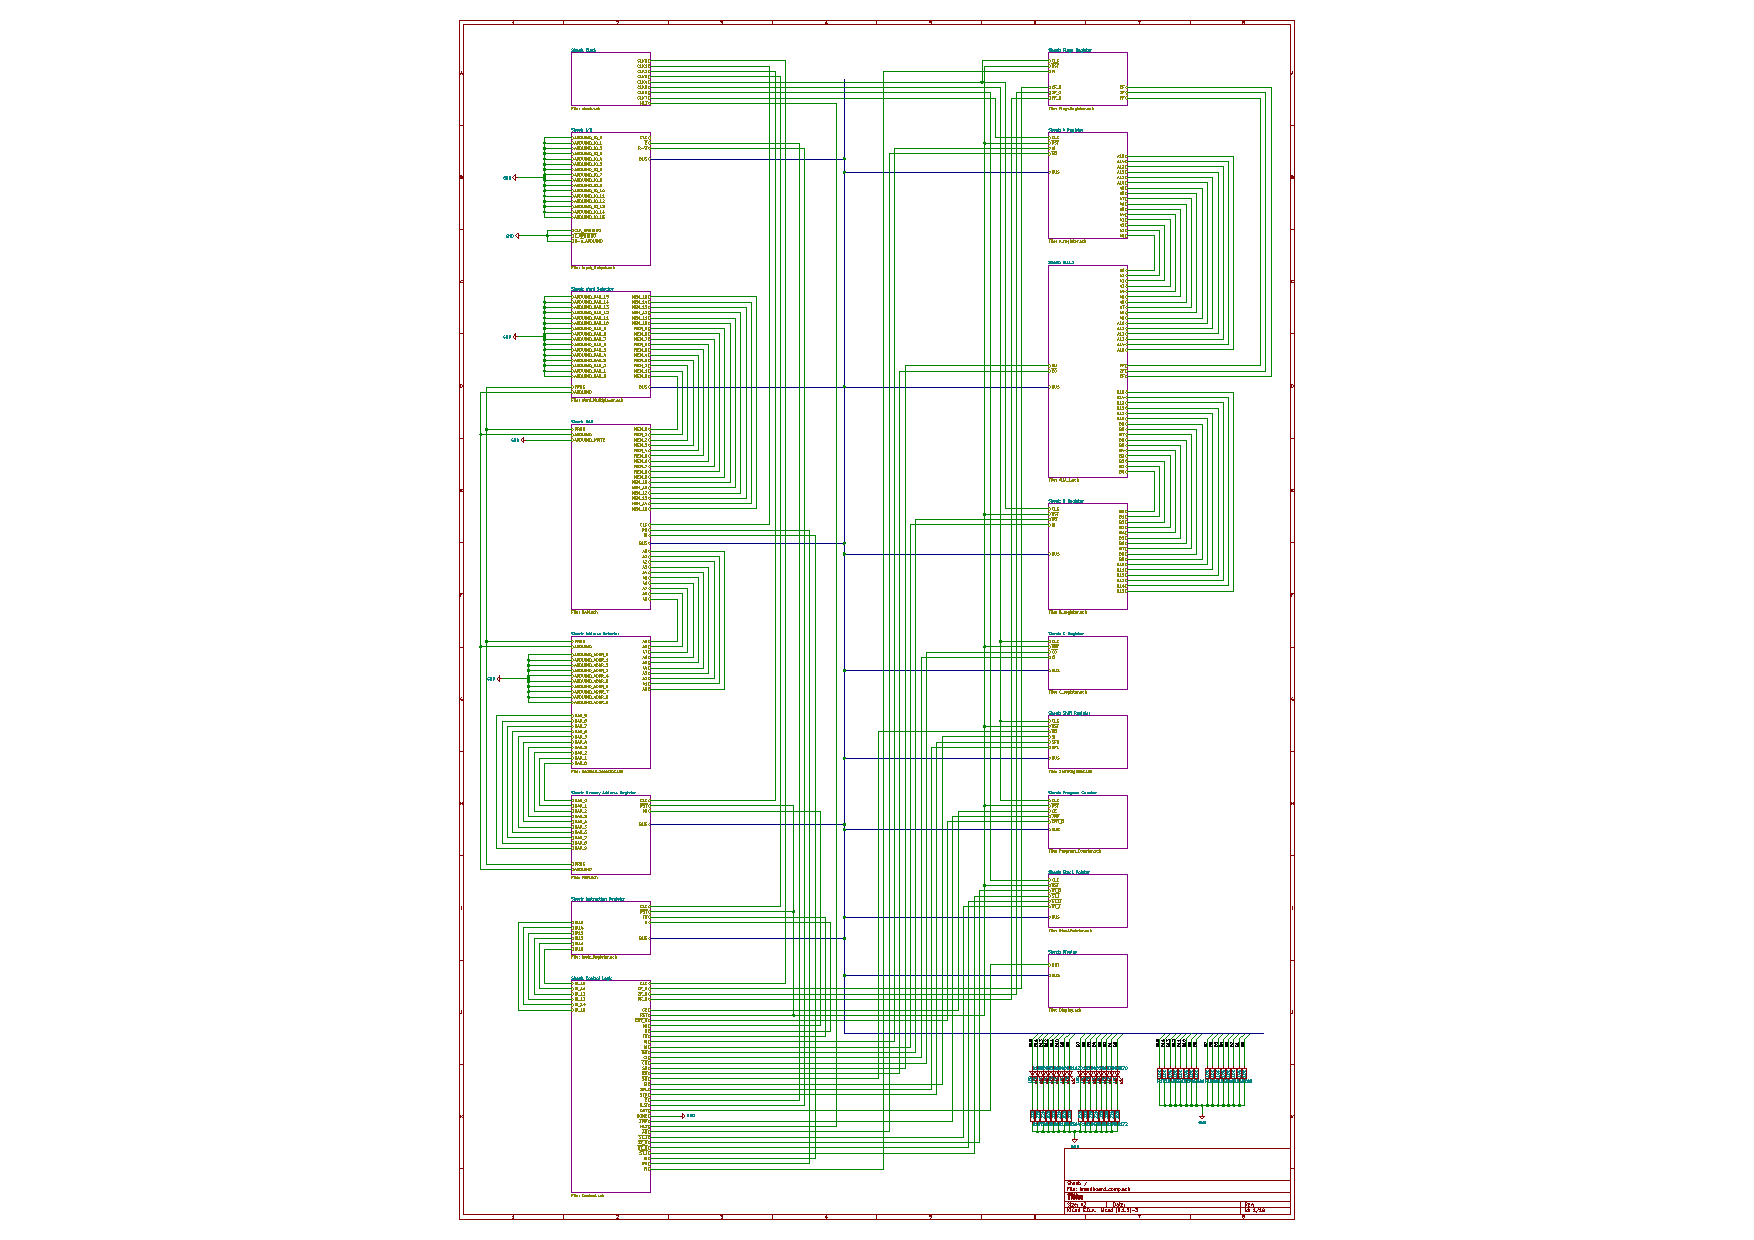
\includepdf[page={9}]{./pdf/kicad}

 \paragraph{Instruction Register} \ref{ir}
 The instruction Register is very similar in construction the the A register \ref{a-reg}, B register \ref{b-reg} and C register
 \ref{c-reg}. It uses two \emph{74LS273} \cite{74ls273} 8-bit flip-flop chips to store one 16-bit word of data, which can be
 latched in from the data bus. It also has two \emph{74LS245} buffer chips used to assert its contents onto the bus when a read
 request is issued. The main difference between the Instruction Register and any other register is the fact that only its 10
 least significand bits are asserted back onto the data bus during a read operation. This is because the Instruction Regsiter
 holds instructions, which are structered as a six-bit \emph{opcode} and a 10-bit \emph{address or immediate operand}. The 6-bit
 \emph{opcode} is connected directly to the \emph{control logic} module. Control Signal processing is handled using a simple
 AND gate.

 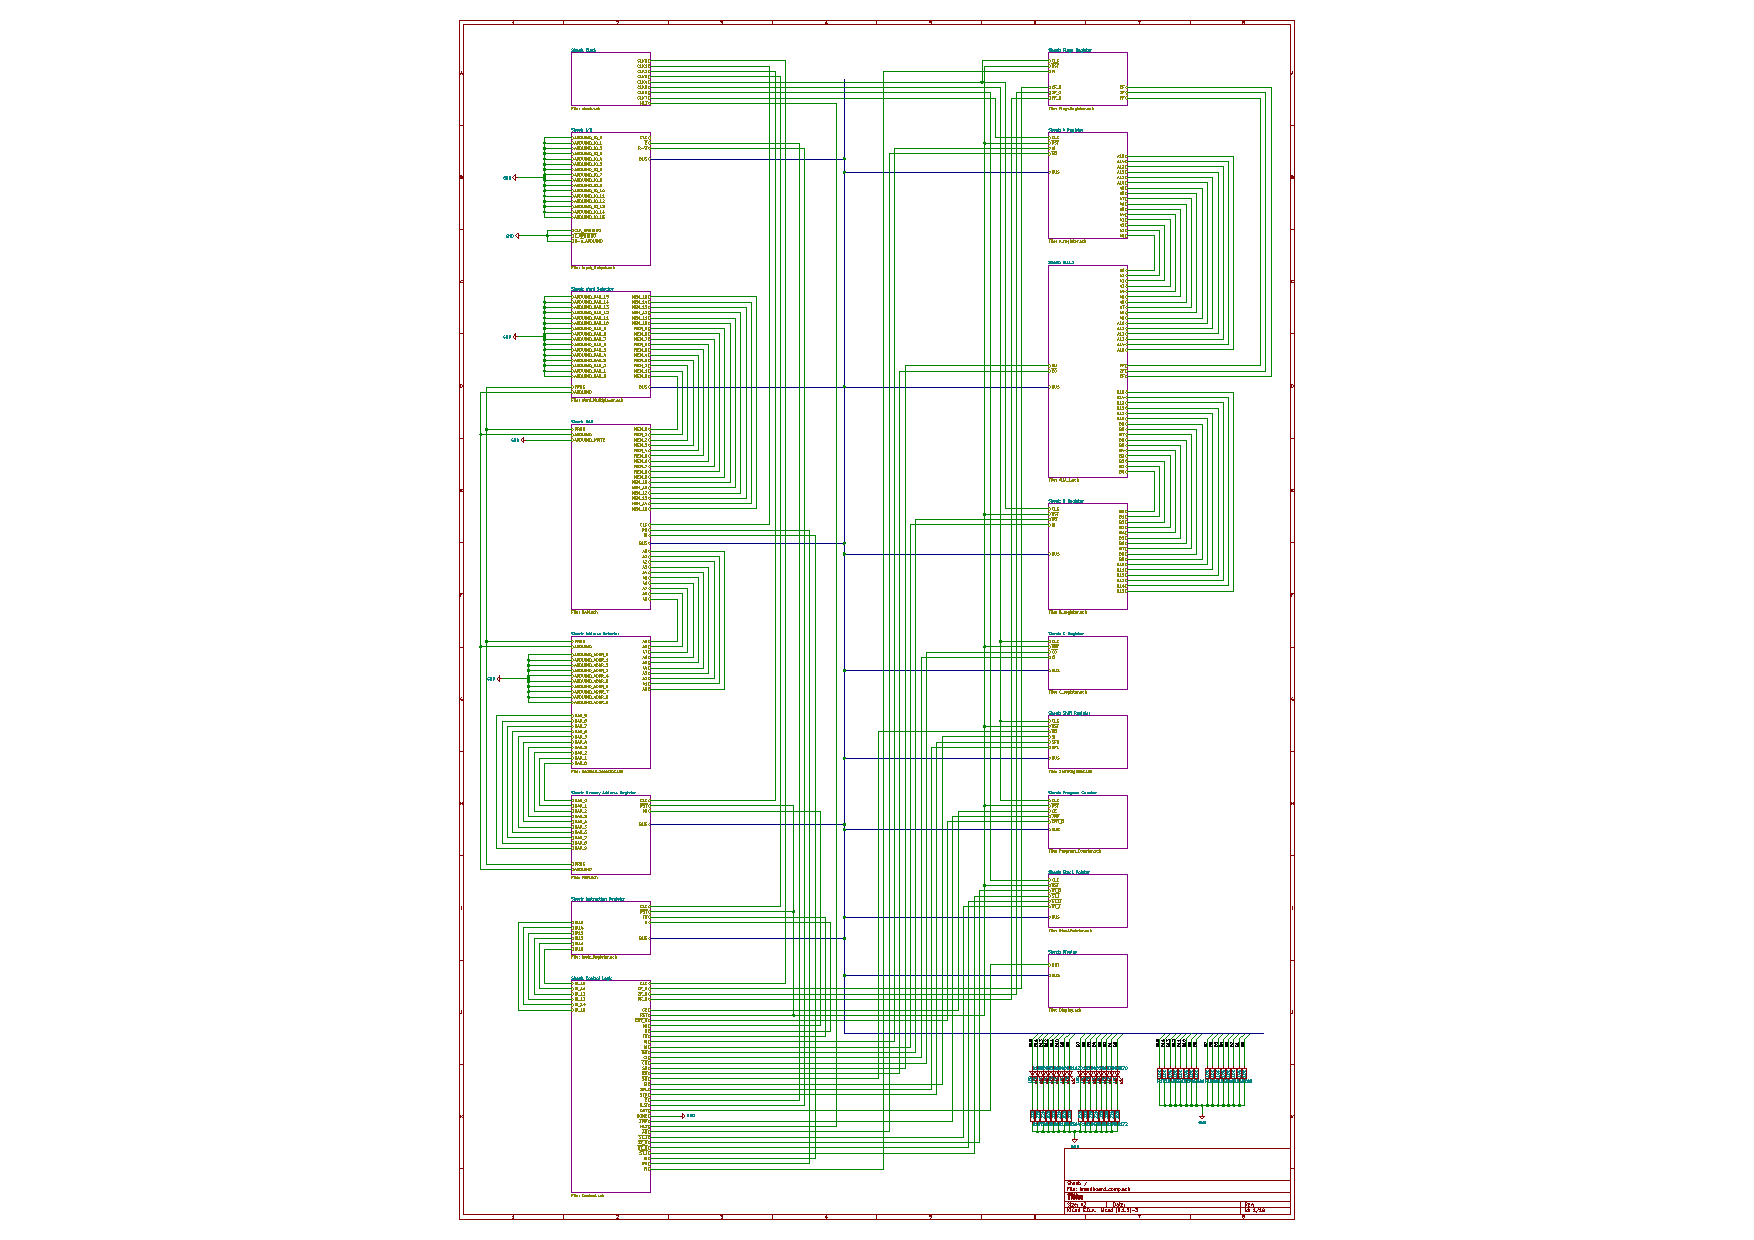
\includepdf[page={18}]{./pdf/kicad}

 \paragraph{Word Selector} \ref{word-select}
 The Word Selector design heavily relies on the \emph{74LS157} data selector chip \cite{74ls157}. A two stage design is proposed.
 The first stage of four selector chips chooses between the data provided by the /emph{DIP switches} and the \emph{Arduino Mega}
 \cite{arduino2020mega}. This stage is handeled by the \emph{ARDUINO} control signal. The output of this selector stage is fed
 forward to the second stage of 4 selector chips. These chips decide wheter to output the programming data provided by the
 previous selectors or the bus data based on the \emph{PROG} signal.

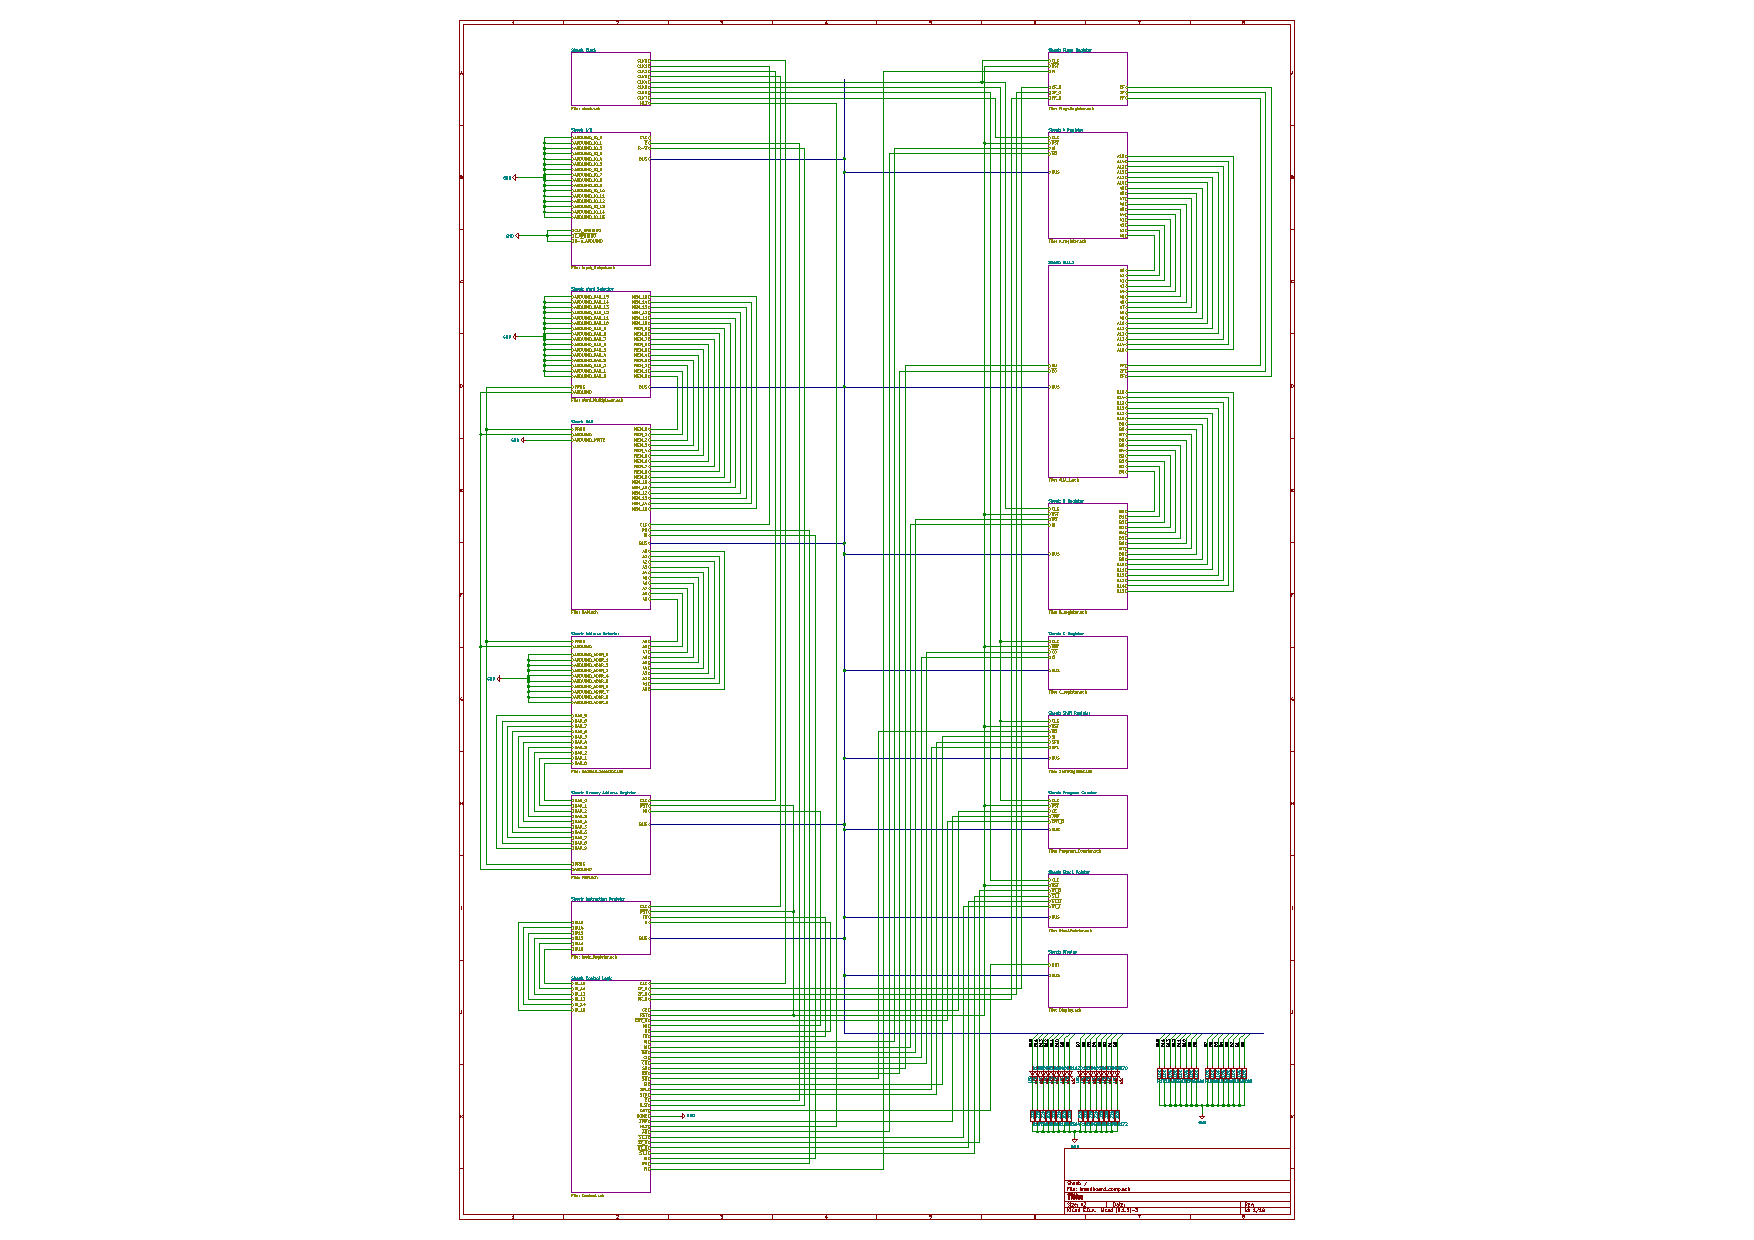
\includepdf[page={15}]{./pdf/kicad}

\paragraph{Address Selector} \ref{addr-select}
The Address selector is designed the same way as the Word Selector described in the previous
paragraph. The main difference is that, since it only has a final output of 10 bits,
each selector stage only contains three \emph{74LS157} \cite{74ls157} selector chips.

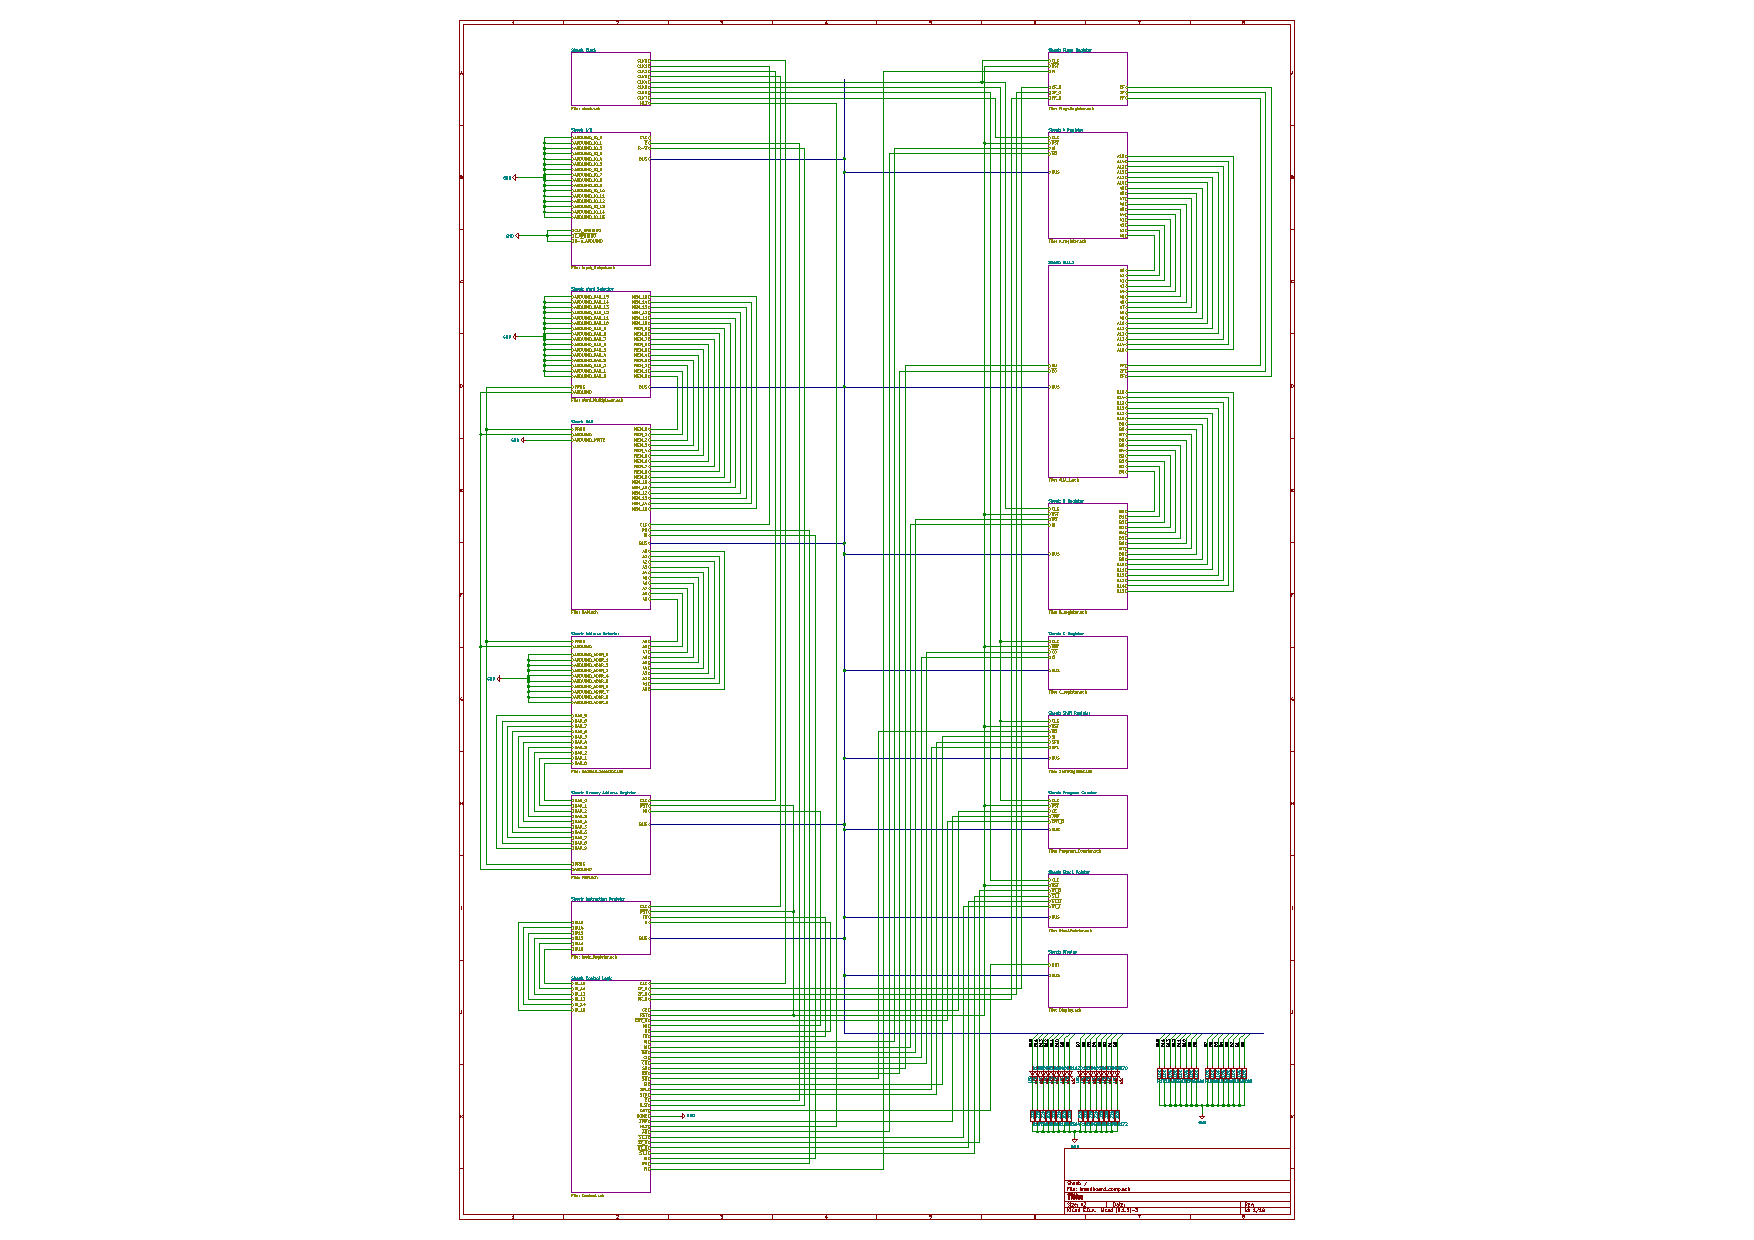
\includepdf[page={8}]{./pdf/kicad}

\paragraph{Control Signals}
The design of the Control Logic module \ref{control-logic} is centered around the \emph{AT28C64B}
EEPROM chip from \emph{Atmel} \cite{at28c64b}. EEPROM stands for \emph{Electronically Erasable
and programmable Read-Only Memory}. Essentially, an EEPROM memory acts as a look-up table.
It's input is an address and the output is a word of data. This can be used as a substitute
for any combinatorial circuit made out of ANDs, ORs, inverters etc.. By choosing an EEPROM,
instead of building a combinatorial circuit, the completed design benefits from multiple
advantages:
\begin{itemize}
  \item \emph{Simplified design:} if a combinatorial circuit would be designed in the place of
  EEPROMS, it would be of a significant size, given the large number of variables (10 binary
  inputs and 31 binary outputs). Such a circuit would not only be very dificult to design and
  physically implement with chips and wires, it would also go against the core design principle
  of simplicity of understanding.
  \item \emph{Easy re-progamming:} EEPROMs can be re-programmed using an of-the-shelf USB
  programmer, a microcontroller like an Arduino \cite{arduino2020mega} or even a simple custom
  built circuit. This makes them especially suitable for application in the design of 16-bit
  breadboard computer as they can easily be removed from the module, reprogrammed to include
  new instructions or modify existing ones and then re-inserted into to rest of the circuit.
  \item \emph{No extra conceptual abstraction}: While the EEPROM chips themselves are much more
  complex chips compared to most of the chips used in other modules (their data sheet doesn't
  provide a transistor diagram or even a low-level diagram, just a high-level block diagram),
  conceptually they don't increase the complexity of the design, since they can be thought of
  as a combinatorial circuit made of simple gates or a memory array made up of rows of registers
  with a selection circuit. As such, the simplicity of both concept and physical implementation
  is maintained.
\end{itemize}
The reasons for choosing this particular EEPROM chip are as follows:
\begin{itemize}
  \item \emph{Parallel Interface: } There are two main types of EEPROMs: parallel and serial. A
  serial interface uses a single pin to transmit addresses and data respecitvley. This poses
  issue to the design of the module since a separate, faster clock and a shift circuit would be
  needed to shift in addresses and shift out data on each clock cycle. This significantly adds
  to the complexity of the entire design. A parallel interface, on the other hand, is much
  easier to work with, since all address bits and all data bits are available at the same time,
  which means they can be accessed synchronously on the same clock cycle.
  \item \emph{Address width: } The \emph{AT28C64B} \cite{at28c64b} is part of a larger family
  of EEPROM chips designed and built by atmel. The main differences between the chips are access
  time and address width. They all have the same data width of 1 byte. Since the plan is to
  run the clock of the breadboard computer at a relatively low frequency (under 1 kHz), the
  access time will not make a significant difference. What is important to consider, though,
  is the address width. The different chips in the Atmel EEPROM Family (AT28C16, AT28C64,
  AT28C256 etc.) have addresses of different widths. The \emph{AT28C64B} \cite{at28c64b}
  offers 13 address bits, enough to accommodate the 10-bit address width of the breadboard
  computer (this requirement will be explained shortly).
  \item \emph{Wide-spread adoption and compatibiliy: } The \emph{AT28C64B} is a widley used chip
  and thoroughly understood chip. As such, it makes interfacing with programmers trivial, as
  most programmers have a profile for it already built in, and it also comes with a plethora
  of online tools, documentation, personal experiences and tips and tricks from other users of
  the chip.
\end{itemize}
The design of the \emph{Control Logic} module \ref{control-logic} makes use of 4 \emph{AT28C64}
chips. Each chip is reasponsible for 8 control signals, with the exception of one chip which
handles only 7 signals (the computer features 31 contol signals without the two clock signals).
The 13 address bits of the EEPROMs are split up into a logical address of 10 bits and a zero-
address of three bits, since only 10 address bits are required by the computer. This 10 bit
address is split up into three components:
\begin{itemize}
  \item \emph{6-bit opcode: } The lowest six bits of the address are the opcode of the
  instruction. These are connected directly from the \emph{Instruction Register} \ref{ir}
  \item \emph{3-bit flags: } The next three bits are the flags which come directly from the
  \emph{Flags register} \ref{flags}
  \item \emph{3-bit time step: } The last three bits form a step counter.
\end{itemize}
The reasoning for including a time-step counter into the address is because of the fact that
each instruction has to execute multiple sequences of control signals to fullfil its task. The
counter is built out of a \emph{74LS161} \cite{74ls161} 4-bit counter chip, from which only the
lowest order three bits are used. These bits are fed into the four eeprom chips, as well as
into a \emph{74LS138} \cite{74ls138}  chip which turns a three bit code into 8 bits, where only
one bit is active at one time. The decoded 8 bits are connected to LEDs to make visually
recognising the current time-step easier. The \emph{74LS161} \cite{74ls161} chip counts based on
the negative, or inverted clock. As a consequence of this, the control logic module has time
between the clock pulses of the main clock to set a new address and then set appropiate control
signal for the next main clock pulse. To make programming of the EEPROM chips easier, all signals
which are active-low are inverted, so that a logic 1 will be programmed if the signal should be
active and a logic zero if the signal should be inactive. Besides this, the \emph{control
signals} module \ref{control-sigs}, which just consists of LEDs on all control signal lines, was
built into this diagram. The final part to discuss on the design of the control logic module is
the reset circuit. Three elements play into the reset circuitry:
\begin{itemize}
  \item \emph{A simple push button}, so that the computer can be manually reset
  \item \emph{The RST control signal}, whih allows the computer to reset itself
  \item \emph{The DONE control signal}, which allows the computer to terminate an instruction
  early, in case it has less then 8 steps.
\end{itemize}
The reset push-button as well as the \emph{RST} signal are combined and together create the
\emph{RST control signal}, which is then spread out to all modules of the computer. Besides this,
this signal is further combined with the \emph{DONE} signal, as this signal, if taken high, should
reset \emph{only} the \emph{74LS161} step counter. \\
This concludes the design of the control logic module.

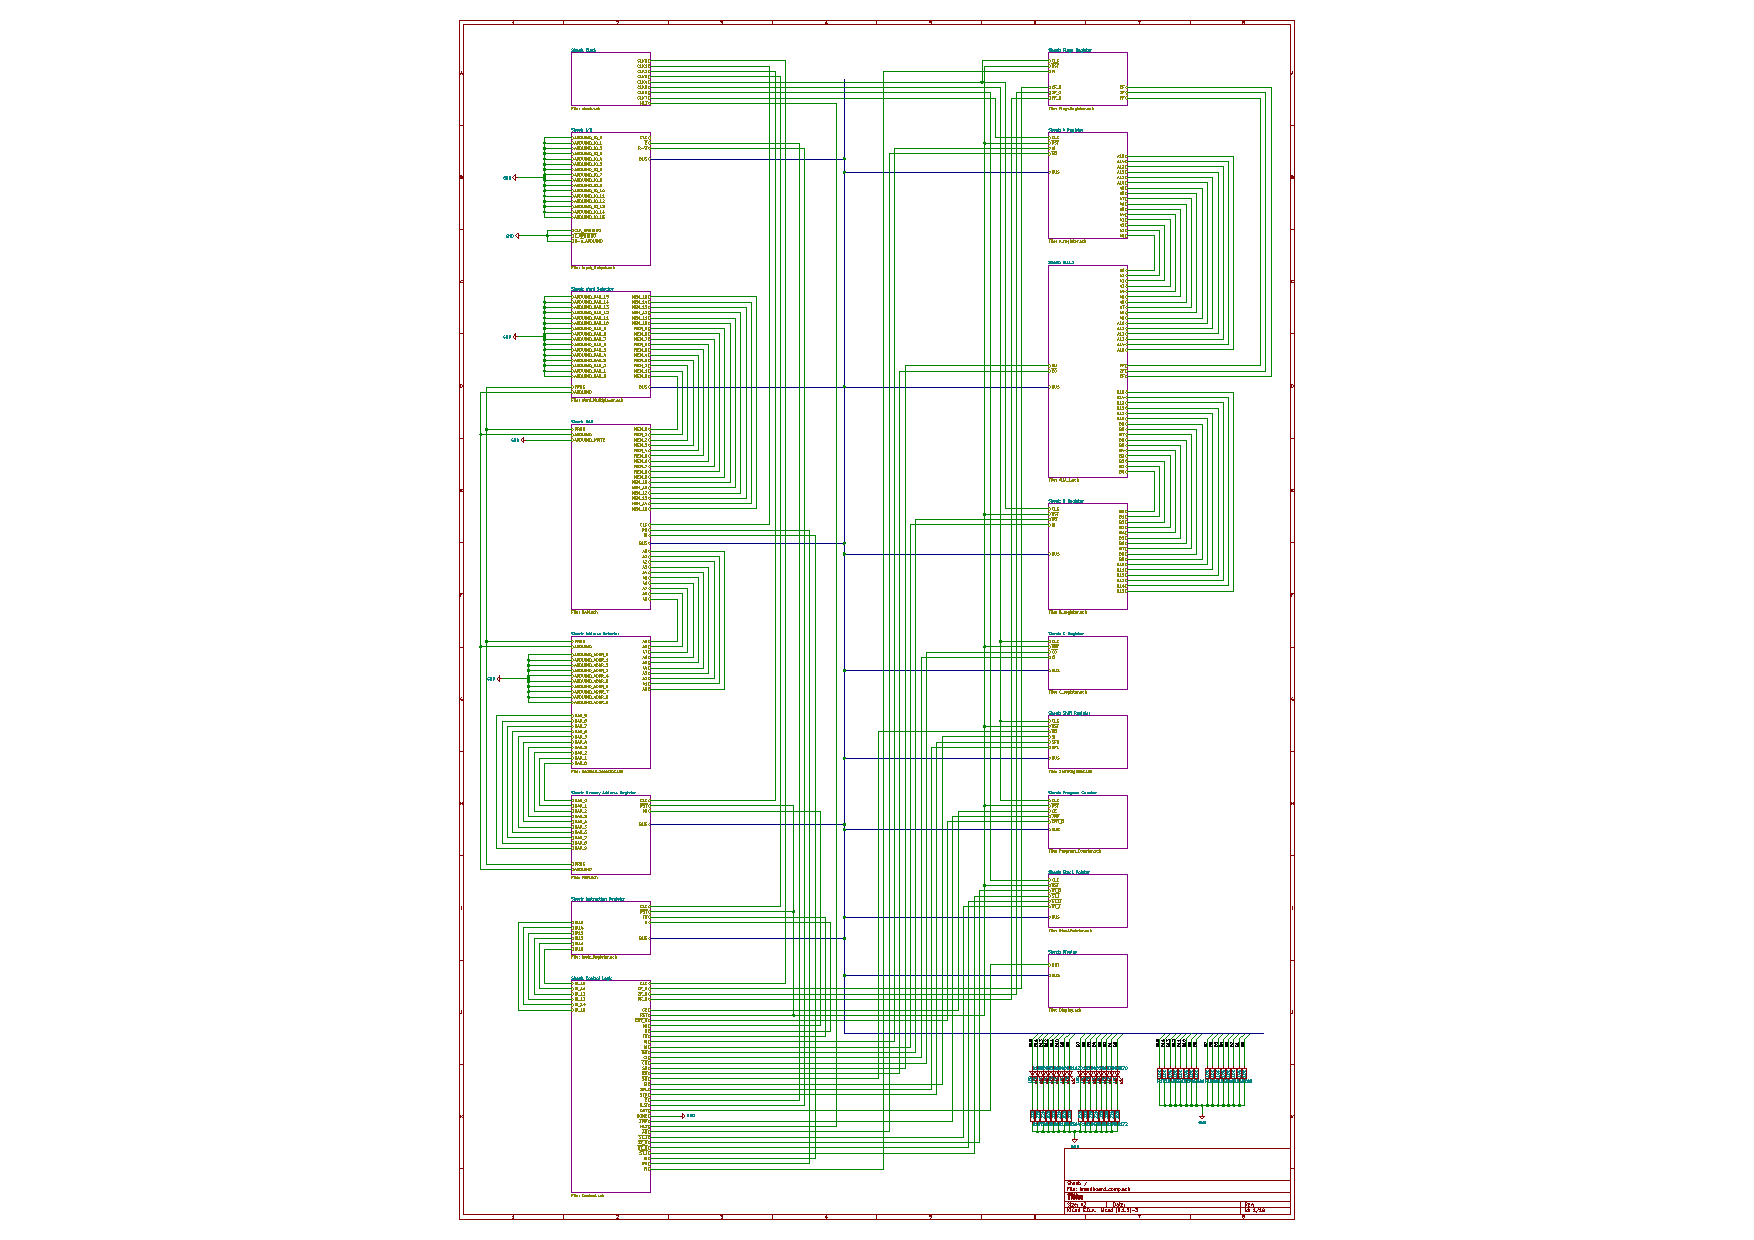
\includepdf[page={16}]{./pdf/kicad}
